%TC:ignore

\textbf{Imperial College London Business School: Template for : Individual Research Report, MS, Business Analytics, 
}

\textbf{Template Disclaimer}

By making use of any template, you agree to the following:

NO WARRANTIES: All of the information provided on this template is provided "AS-IS" and with NO WARRANTIES. No express or implied warranties of any type, including for example implied warranties of merchantability or fitness for a particular purpose, are made with respect to the information, or any use of the information, on this template. Parties involved in preparing the template makes no representations and extends no warranties of any type as to the accuracy or completeness of any information or content on this template.


DISCLAIMER OF LIABILITY: All parties involved in preparing the document specifically DISCLAIMS LIABILITY FOR INCIDENTAL OR CONSEQUENTIAL DAMAGES OF ANY KIND and assumes no responsibility or liability for any loss or damage suffered as a result of the use or misuse of any of the information or content in this template. The parties involved in preparing the document assumes or undertakes NO LIABILITY for any loss or damage suffered as a result of the use, misuse or reliance on the information and content on this template. Use at your own risk.

{\color{red} \rule{\linewidth}{0.5mm} }
\textcolor{red}{\textbf{COMMENT THE FOLLOWING LINES IN THE TEMPLATE TO HIDE HOW-TO SECTION}}
\begin{verbatim}
\section{How to use this template (Comment section before use)}
%TC:ignore

\textbf{Imperial College London Business School: Template for : Individual Research Report, MS, Business Analytics, 
}

\textbf{Template Disclaimer}

By making use of any template, you agree to the following:

NO WARRANTIES: All of the information provided on this template is provided "AS-IS" and with NO WARRANTIES. No express or implied warranties of any type, including for example implied warranties of merchantability or fitness for a particular purpose, are made with respect to the information, or any use of the information, on this template. Parties involved in preparing the template makes no representations and extends no warranties of any type as to the accuracy or completeness of any information or content on this template.


DISCLAIMER OF LIABILITY: All parties involved in preparing the document specifically DISCLAIMS LIABILITY FOR INCIDENTAL OR CONSEQUENTIAL DAMAGES OF ANY KIND and assumes no responsibility or liability for any loss or damage suffered as a result of the use or misuse of any of the information or content in this template. The parties involved in preparing the document assumes or undertakes NO LIABILITY for any loss or damage suffered as a result of the use, misuse or reliance on the information and content on this template. Use at your own risk.

{\color{red} \rule{\linewidth}{0.5mm} }
\textcolor{red}{\textbf{COMMENT THE FOLLOWING LINES IN THE TEMPLATE TO HIDE HOW-TO SECTION}}
\begin{verbatim}
\section{How to use this template (Comment section before use)}
%TC:ignore

\textbf{Imperial College London Business School: Template for : Individual Research Report, MS, Business Analytics, 
}

\textbf{Template Disclaimer}

By making use of any template, you agree to the following:

NO WARRANTIES: All of the information provided on this template is provided "AS-IS" and with NO WARRANTIES. No express or implied warranties of any type, including for example implied warranties of merchantability or fitness for a particular purpose, are made with respect to the information, or any use of the information, on this template. Parties involved in preparing the template makes no representations and extends no warranties of any type as to the accuracy or completeness of any information or content on this template.


DISCLAIMER OF LIABILITY: All parties involved in preparing the document specifically DISCLAIMS LIABILITY FOR INCIDENTAL OR CONSEQUENTIAL DAMAGES OF ANY KIND and assumes no responsibility or liability for any loss or damage suffered as a result of the use or misuse of any of the information or content in this template. The parties involved in preparing the document assumes or undertakes NO LIABILITY for any loss or damage suffered as a result of the use, misuse or reliance on the information and content on this template. Use at your own risk.

{\color{red} \rule{\linewidth}{0.5mm} }
\textcolor{red}{\textbf{COMMENT THE FOLLOWING LINES IN THE TEMPLATE TO HIDE HOW-TO SECTION}}
\begin{verbatim}
\section{How to use this template (Comment section before use)}
%TC:ignore

\textbf{Imperial College London Business School: Template for : Individual Research Report, MS, Business Analytics, 
}

\textbf{Template Disclaimer}

By making use of any template, you agree to the following:

NO WARRANTIES: All of the information provided on this template is provided "AS-IS" and with NO WARRANTIES. No express or implied warranties of any type, including for example implied warranties of merchantability or fitness for a particular purpose, are made with respect to the information, or any use of the information, on this template. Parties involved in preparing the template makes no representations and extends no warranties of any type as to the accuracy or completeness of any information or content on this template.


DISCLAIMER OF LIABILITY: All parties involved in preparing the document specifically DISCLAIMS LIABILITY FOR INCIDENTAL OR CONSEQUENTIAL DAMAGES OF ANY KIND and assumes no responsibility or liability for any loss or damage suffered as a result of the use or misuse of any of the information or content in this template. The parties involved in preparing the document assumes or undertakes NO LIABILITY for any loss or damage suffered as a result of the use, misuse or reliance on the information and content on this template. Use at your own risk.

{\color{red} \rule{\linewidth}{0.5mm} }
\textcolor{red}{\textbf{COMMENT THE FOLLOWING LINES IN THE TEMPLATE TO HIDE HOW-TO SECTION}}
\begin{verbatim}
\section{How to use this template (Comment section before use)}
\input{howtouse.tex}
\pagebreak
\end{verbatim}
{\color{red} \rule{\linewidth}{0.5mm}}

\textcolor{red}{\textbf{FONT USAGE}}

The Arial font is recommended for the Individual Research Report. However, this needs to be installed manually as discussed in this document. For Overleaf, Helvetica has been used. If you are able to install Arial, comment the line \texttt{usepackage[scaled]\{helvet\}} and uncomment \texttt{usepackage\{uarial\}}.

{\color{red} \rule{\linewidth}{0.5mm}}

\textbf{FORMATTING AND PAGE NUMBERING CONVENTIONS USED}

\begin{itemize}
	\item Geometry
	\begin{itemize}
		\item left-hand margin of 4 cm;
		\item right-hand margin of 2.5cm (1 inch);
		\item top margin 2.5cm (1 inch);
		\item bottom margin 2.5cm (1 inch).
	\end{itemize}
	\begin{itemize}
		\item The Synopsis, Acknowledgements, List of Contents and Notation should be numbered with upper case Roman Numerals.
		\item The main text, starting with the first page of the first chapter (or Introduction) should be numbered, starting with page 1, using Arabic Numerals, through to the end of the references.
		\item \textbf{Appendices should be numbered using lower case Roman Numerals. -- Check to make sure this is what is needed. If not comment \texttt{\\pagenumbering\{roman\}} in template before Appendix}
	\end{itemize}
	\item Pages must be numbered at the bottom centre of the page.
	\item The title page should be blank.
\end{itemize}

\subsection{Prerequisites}

There are 2 primary pre-requisites: First, to install the Bath BibTeX style and second to install the Arial font. Note that if Arial cannot be installed, it may be possible to use Helvetica if the department agrees 

\textbf{1. Install the Bath BibTeX style (See Included Folder)}

\textbf{2. Install Font Arial}: See \hyperlink{https://www.tug.org/fonts/getnonfreefonts/}{https://www.tug.org/fonts/getnonfreefonts/} and 

\textbf{Notes from \hyperlink{https://tex.stackexchange.com/questions/37120/how-can-i-install-uarial-sty-on-a-mac}{Install uarial on a Mac} question on Stackexchange: }

The font can be easily installed via the script getnonfreefonts. It is available at tug.org: \hyperlink{http://www.tug.org/fonts/getnonfreefonts/}{getnonfreefonts}. I tried the installation of \hyperlink{http://www.tug.org/fonts/getnonfreefonts/install-getnonfreefonts}{getnonfreefonts} on my Mac.

\begin{itemize}
	\item Install MacTeX 
	\item Download the installation script. Open the terminal and go to the folder Download
	
	\texttt{cd Download}
	\item Run the installation: \texttt{sudo texlua install-getnonfreefonts}
	
	The installation finished and the scipts with their execute files getnonefreefonts and getnonfreefonts-sys are now located at \texttt{/usr/local/texlive/2011/bin/x86\_64-darwin/}
	
	\item Now you can run the script \texttt{sudo getnonfreefonts-sys -a}
\end{itemize}

\subsection{Images}
\begin{figure*}[!ht]
	\centering
	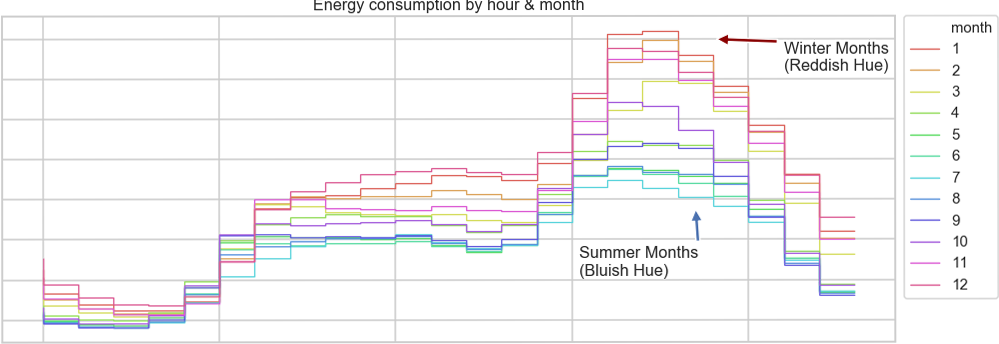
\includegraphics[width=16cm]{images/testimage1}
	\caption{This is an image}
	\label{fig:testimage1}
\end{figure*}

\begin{figure*}[!ht]
	\centering
	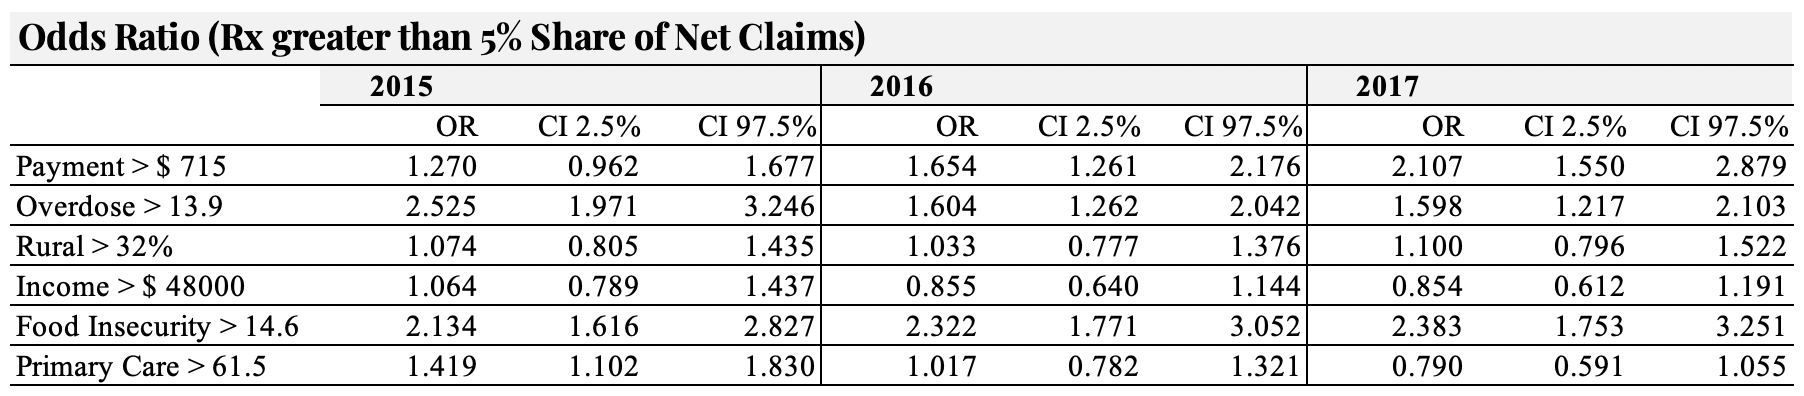
\includegraphics[width=16cm]{images/testimage2}
	%	\caption{Round 1 Blue Strategy to increase Market Share}
	\captionof{table}[This is a table shown as an image]{This is a table shown as an image}
	\label{fig:testimage2}
\end{figure*}

\begin{figure*}[!ht]
	\centering
	\subfloat[A floating image]{{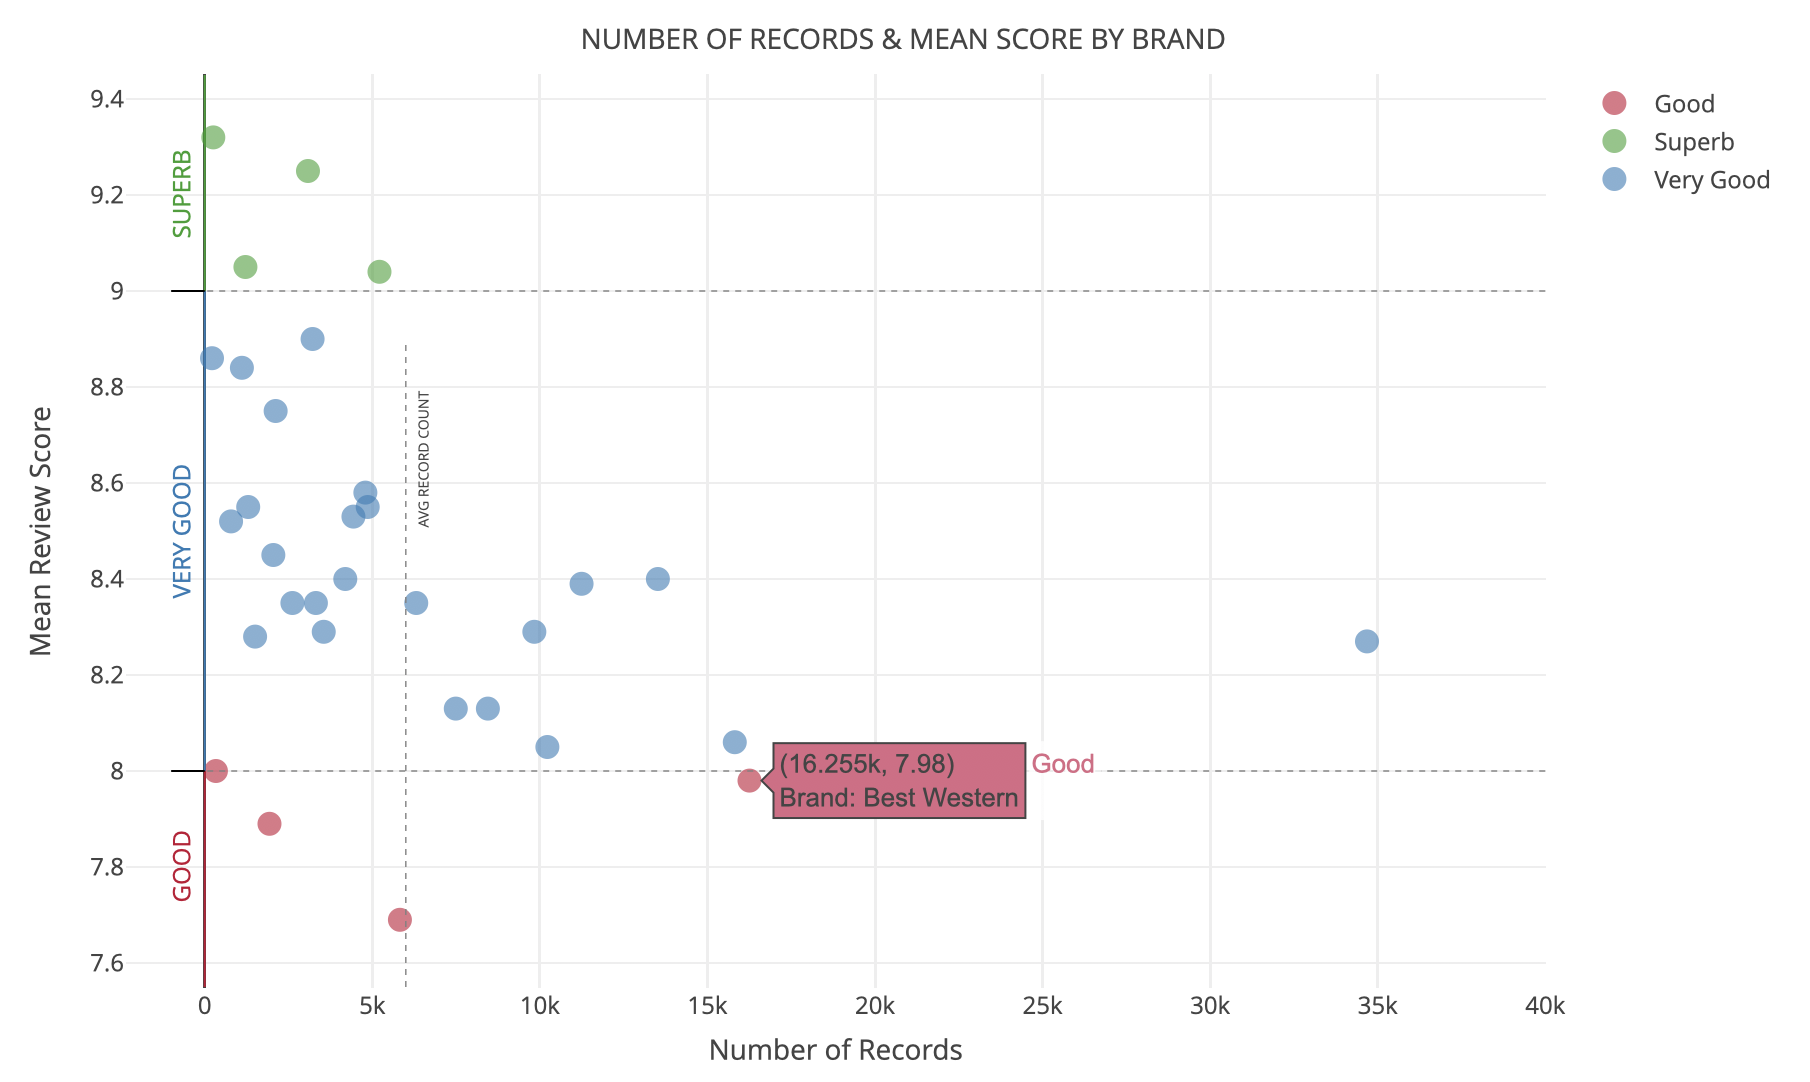
\includegraphics[width=7.2cm]{images/testimage3_1} }}%
	%	\qquad
	\subfloat[Another image ]{{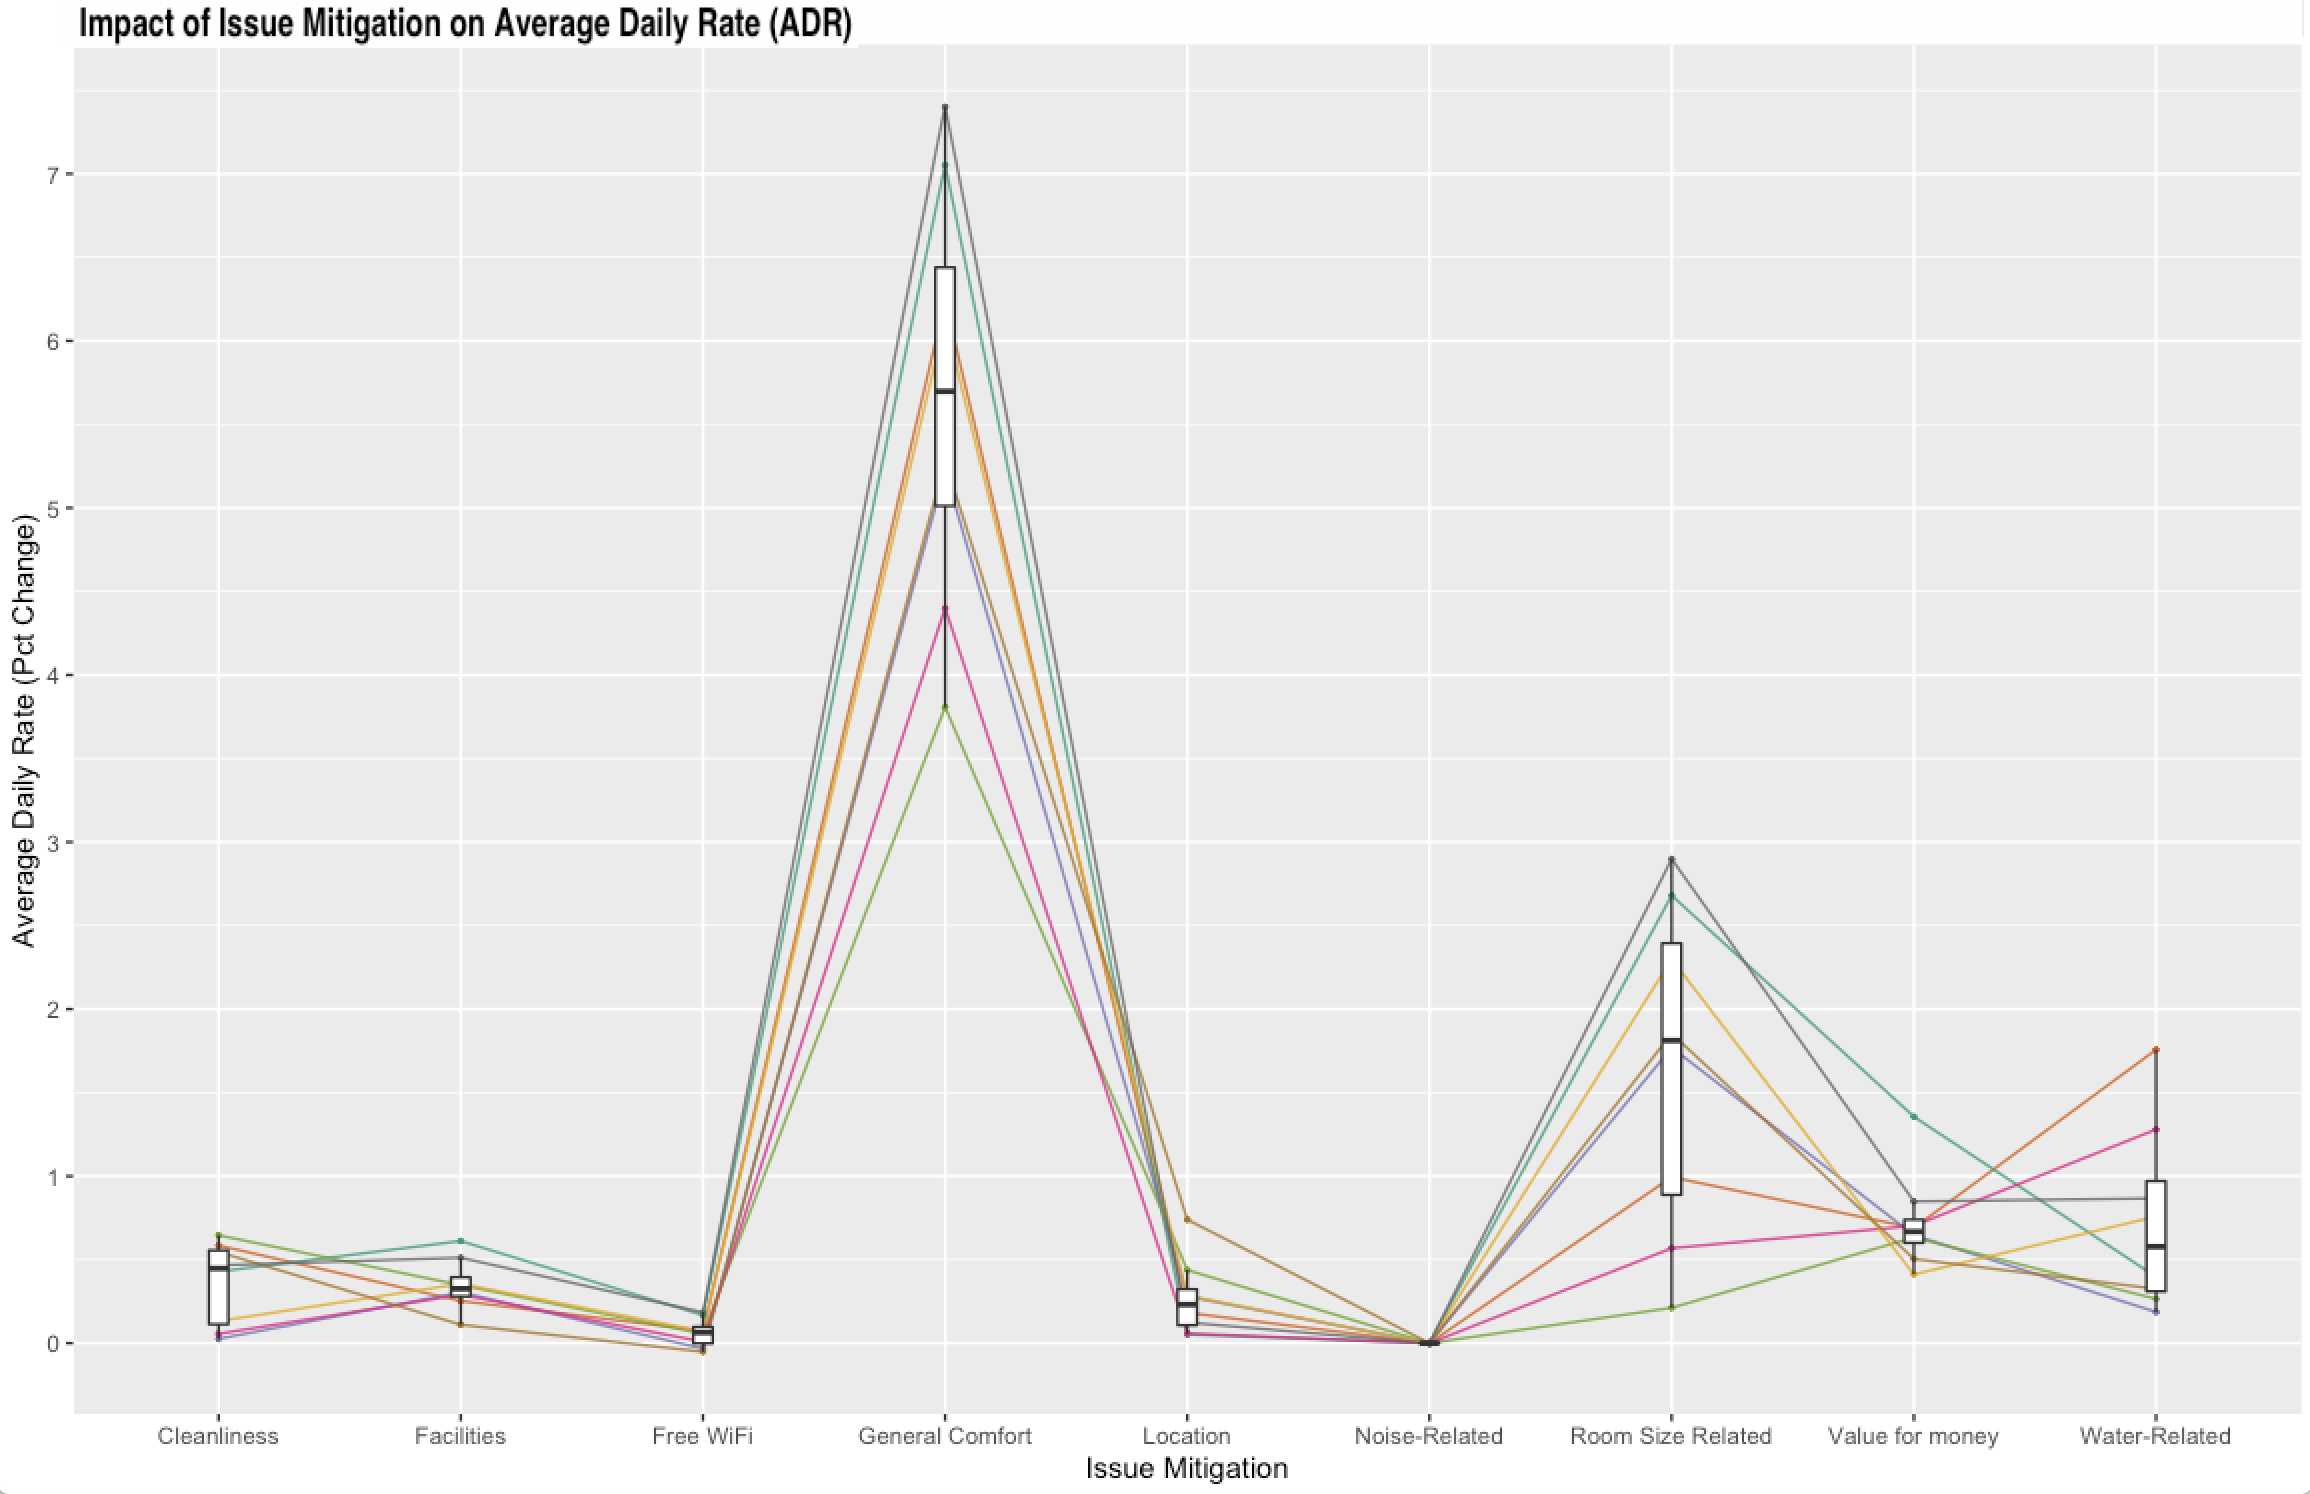
\includegraphics[width=7.2cm]{images/testimage3_2}}}%
	\caption{Floating Images}%
	\label{fig:floatimage}%
\end{figure*}


\subsection{Miscellaneous}

\subsubsection{Hyperlinks}
% HYPERLINK
\href{https://www.cnn.com}{A hyperlink to CNN.com}

% TO ADD A REFERENCE TO A SECTION
This is a section labelled as "sec1"
\label{sec:sec1}

This is a reference to the section sec1: \ref{sec:sec1}

\fbox{\begin{minipage}{43em}
		\textbf{Using fbox and minipage}\\
Text enclosed in a box
\end{minipage}}

% CODE
\subsubsection{Python Code Formatting}
\lstinputlisting[language=Python]{code/test.py}

\subsubsection{R Code Formatting}
\lstinputlisting[language=R]{code/test.R}

\subsubsection{Tables and Equations}

Examples with tables, caption centering, equations and aligned equations.

\begin{table}[!ht]
	\centering
	\captionsetup{justification=centering}
	\begin{tabular}{l|llrr}
		%		\hline
		\textbf{Model}            & \textbf{Parameter} & \textbf{Best Fit}              & \textbf{Train RMSE}             & \textbf{Test RMSE}               \\ \hline
		Linear Regression         & -                  & -                              & \rupee16,758,137 & \rupee57,778,006  \\ \hline
		Random GLM                & maxOrder           & maxInt.Order = 2        & \rupee15,551,472 & \rupee100,219,602 \\ \hline
		SVM RBF Kernel            & C, Sigma           & sigma = 26.76, C = 4     & \rupee17,075,271 & \rupee34,932,347  \\ \hline
		KNN                       & k                  & k = 5                          & \rupee12,255,888 & \rupee54,935,698  \\ \hline
		RandomForest              & mtry               & mtry = 2                       & \rupee8,724,815  & \rupee53,453,612  \\ \hline
		\rowcolor[HTML]{EFEFEF} 
		XGBoost & misc*              & max\_depth = 3, $\eta$ = 0.3, $\gamma$ = 0      & \rupee4,924,454  & \rupee65,211,901  \\ \hline
	\end{tabular}
	\caption{This is a table}
	\label{tab:state_pred}
\end{table}

Split Line in Equations
\begin{equation}
\begin{split}
\label{eqn:natsec}
ln(GVA_{Sector}) = \beta_1ln(SumOfLights)_{t}+\beta_2ln(SumElectricity)_t +\\ \beta_3ln(SumOfLightsSq)_{t} + \beta_4ln(Population)_{t} +
\alpha_i + u_{it}
\end{split}
\end{equation}

Aligned Equations
$$
\begin{aligned}
y_t &= 10.3009 -0.0042x_L - 0.0045x_B - 0.0032x_c -0.0046x_{d1} + \ldots + 0.0176x_{d6} + \eta_t \\
\eta_t &= 0.9146\eta_{t-1} + \epsilon_t -0.5015\epsilon_{t-1}\\
\epsilon_t &= \sim \text{NID}(0,0.003443)
\end{aligned}
$$

\subsubsection{Citations}
This template uses Bath BibTeX: \hyperlink{https://ctan.org/pkg/bath-bst?lang=en}{https://ctan.org/pkg/bath-bst?lang=en}

See: \hyperlink{https://github.com/alex-ball/bathbib/tree/master/bst}{https://github.com/alex-ball/bathbib/tree/master/bst}

This is a citation \citep{Elvidge_Baugh_Zhizhin_Hsu_Ghosh_2017} using \texttt{citep}.

This is a citation \cite{Tibshirani_1996} using \texttt{cite}

%TC:endignore
\pagebreak
\end{verbatim}
{\color{red} \rule{\linewidth}{0.5mm}}

\textcolor{red}{\textbf{FONT USAGE}}

The Arial font is recommended for the Individual Research Report. However, this needs to be installed manually as discussed in this document. For Overleaf, Helvetica has been used. If you are able to install Arial, comment the line \texttt{usepackage[scaled]\{helvet\}} and uncomment \texttt{usepackage\{uarial\}}.

{\color{red} \rule{\linewidth}{0.5mm}}

\textbf{FORMATTING AND PAGE NUMBERING CONVENTIONS USED}

\begin{itemize}
	\item Geometry
	\begin{itemize}
		\item left-hand margin of 4 cm;
		\item right-hand margin of 2.5cm (1 inch);
		\item top margin 2.5cm (1 inch);
		\item bottom margin 2.5cm (1 inch).
	\end{itemize}
	\begin{itemize}
		\item The Synopsis, Acknowledgements, List of Contents and Notation should be numbered with upper case Roman Numerals.
		\item The main text, starting with the first page of the first chapter (or Introduction) should be numbered, starting with page 1, using Arabic Numerals, through to the end of the references.
		\item \textbf{Appendices should be numbered using lower case Roman Numerals. -- Check to make sure this is what is needed. If not comment \texttt{\\pagenumbering\{roman\}} in template before Appendix}
	\end{itemize}
	\item Pages must be numbered at the bottom centre of the page.
	\item The title page should be blank.
\end{itemize}

\subsection{Prerequisites}

There are 2 primary pre-requisites: First, to install the Bath BibTeX style and second to install the Arial font. Note that if Arial cannot be installed, it may be possible to use Helvetica if the department agrees 

\textbf{1. Install the Bath BibTeX style (See Included Folder)}

\textbf{2. Install Font Arial}: See \hyperlink{https://www.tug.org/fonts/getnonfreefonts/}{https://www.tug.org/fonts/getnonfreefonts/} and 

\textbf{Notes from \hyperlink{https://tex.stackexchange.com/questions/37120/how-can-i-install-uarial-sty-on-a-mac}{Install uarial on a Mac} question on Stackexchange: }

The font can be easily installed via the script getnonfreefonts. It is available at tug.org: \hyperlink{http://www.tug.org/fonts/getnonfreefonts/}{getnonfreefonts}. I tried the installation of \hyperlink{http://www.tug.org/fonts/getnonfreefonts/install-getnonfreefonts}{getnonfreefonts} on my Mac.

\begin{itemize}
	\item Install MacTeX 
	\item Download the installation script. Open the terminal and go to the folder Download
	
	\texttt{cd Download}
	\item Run the installation: \texttt{sudo texlua install-getnonfreefonts}
	
	The installation finished and the scipts with their execute files getnonefreefonts and getnonfreefonts-sys are now located at \texttt{/usr/local/texlive/2011/bin/x86\_64-darwin/}
	
	\item Now you can run the script \texttt{sudo getnonfreefonts-sys -a}
\end{itemize}

\subsection{Images}
\begin{figure*}[!ht]
	\centering
	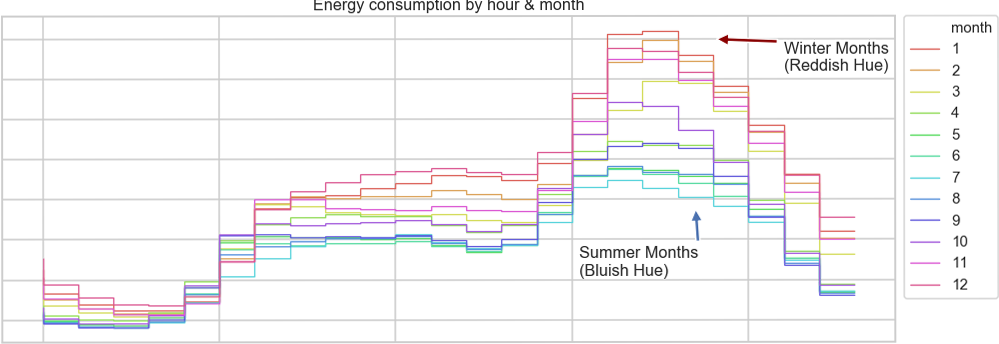
\includegraphics[width=16cm]{images/testimage1}
	\caption{This is an image}
	\label{fig:testimage1}
\end{figure*}

\begin{figure*}[!ht]
	\centering
	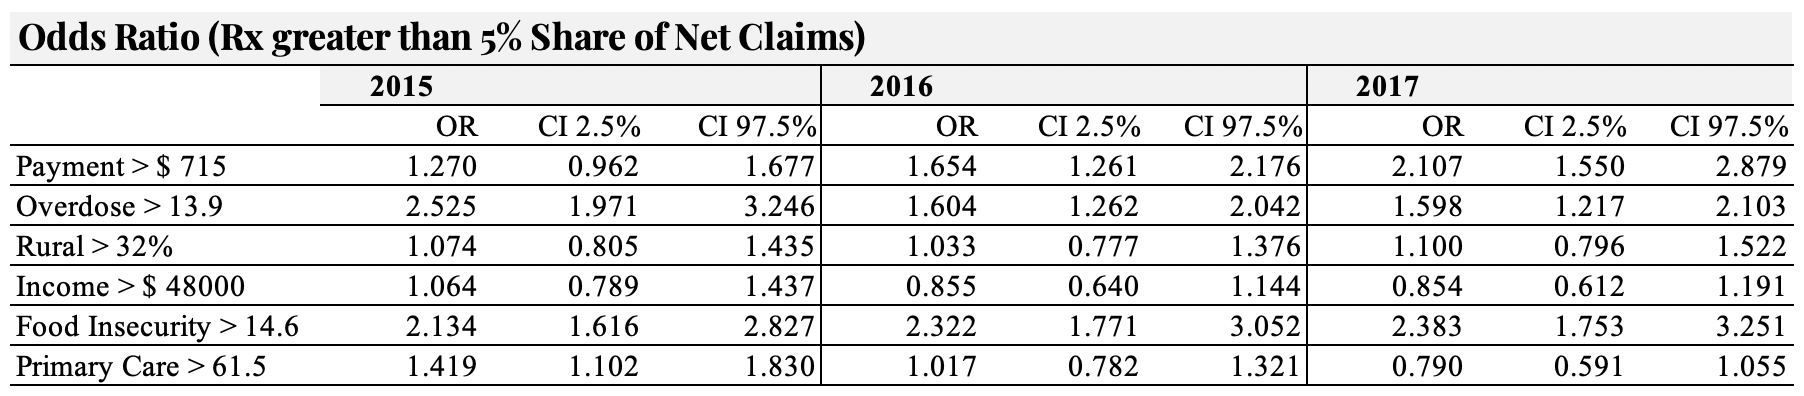
\includegraphics[width=16cm]{images/testimage2}
	%	\caption{Round 1 Blue Strategy to increase Market Share}
	\captionof{table}[This is a table shown as an image]{This is a table shown as an image}
	\label{fig:testimage2}
\end{figure*}

\begin{figure*}[!ht]
	\centering
	\subfloat[A floating image]{{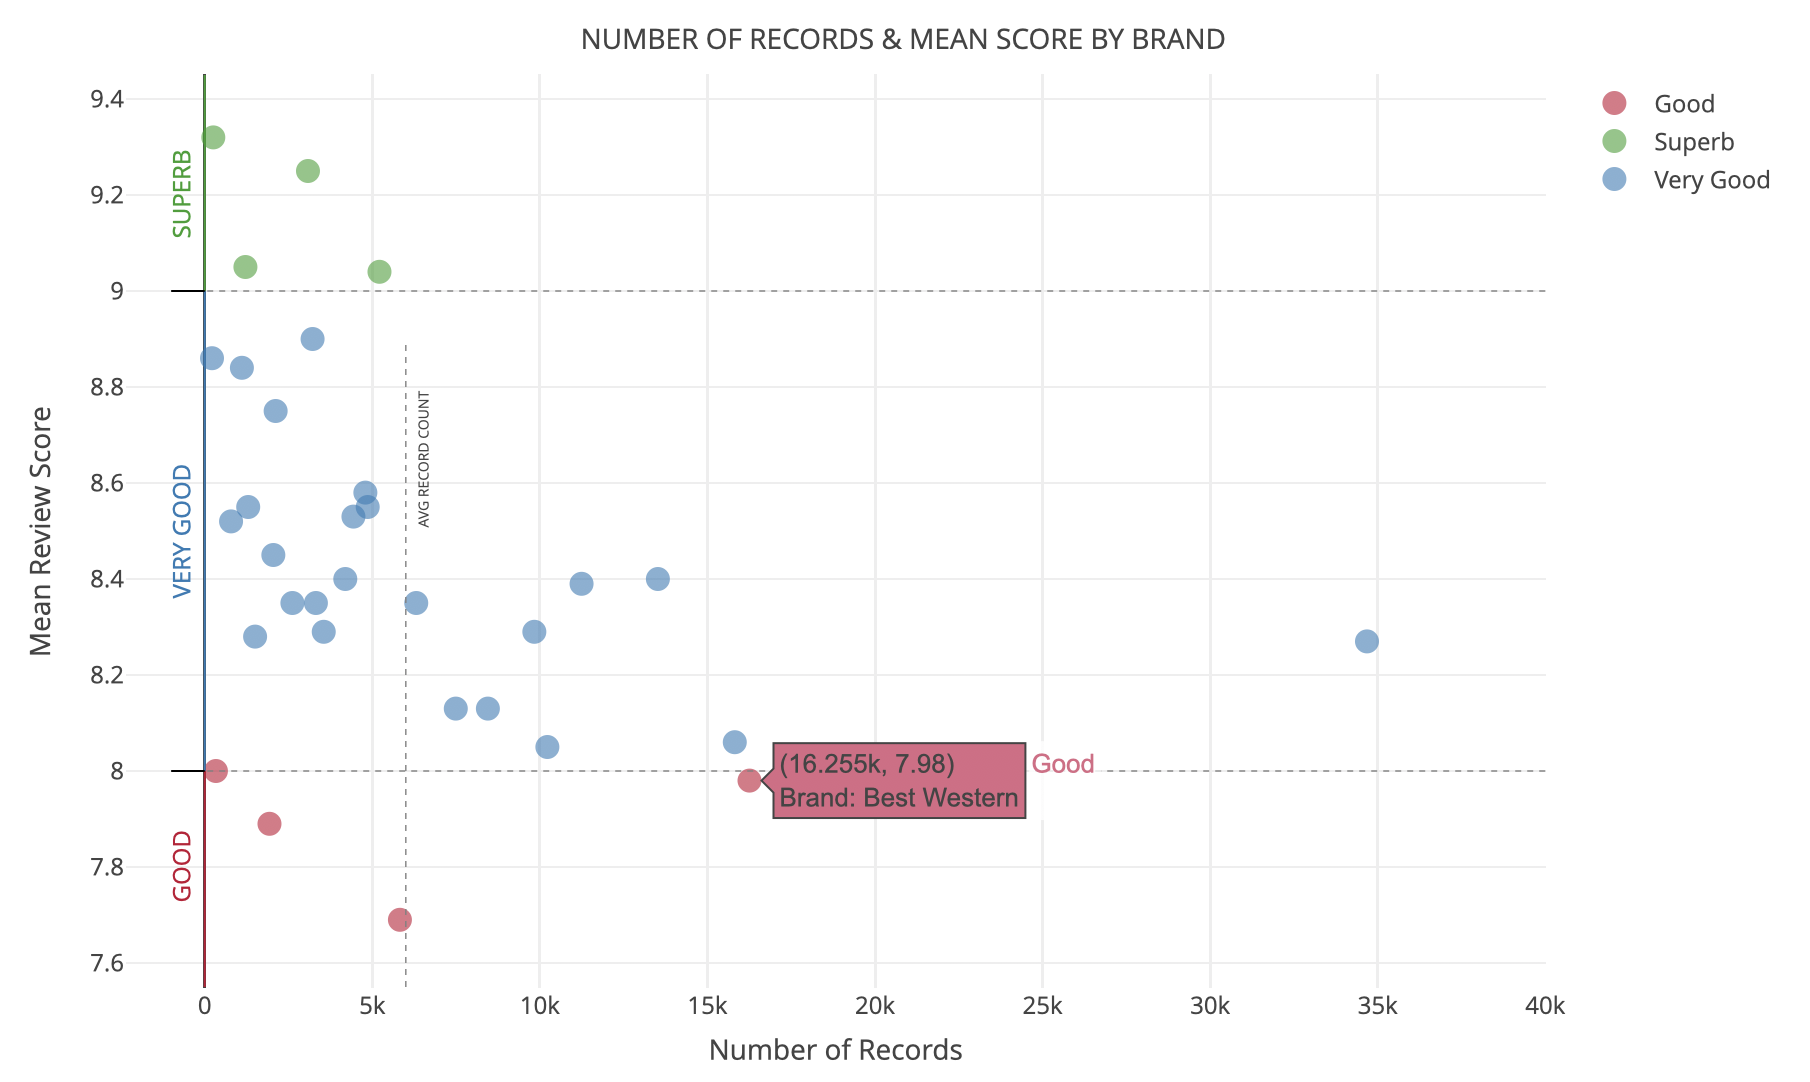
\includegraphics[width=7.2cm]{images/testimage3_1} }}%
	%	\qquad
	\subfloat[Another image ]{{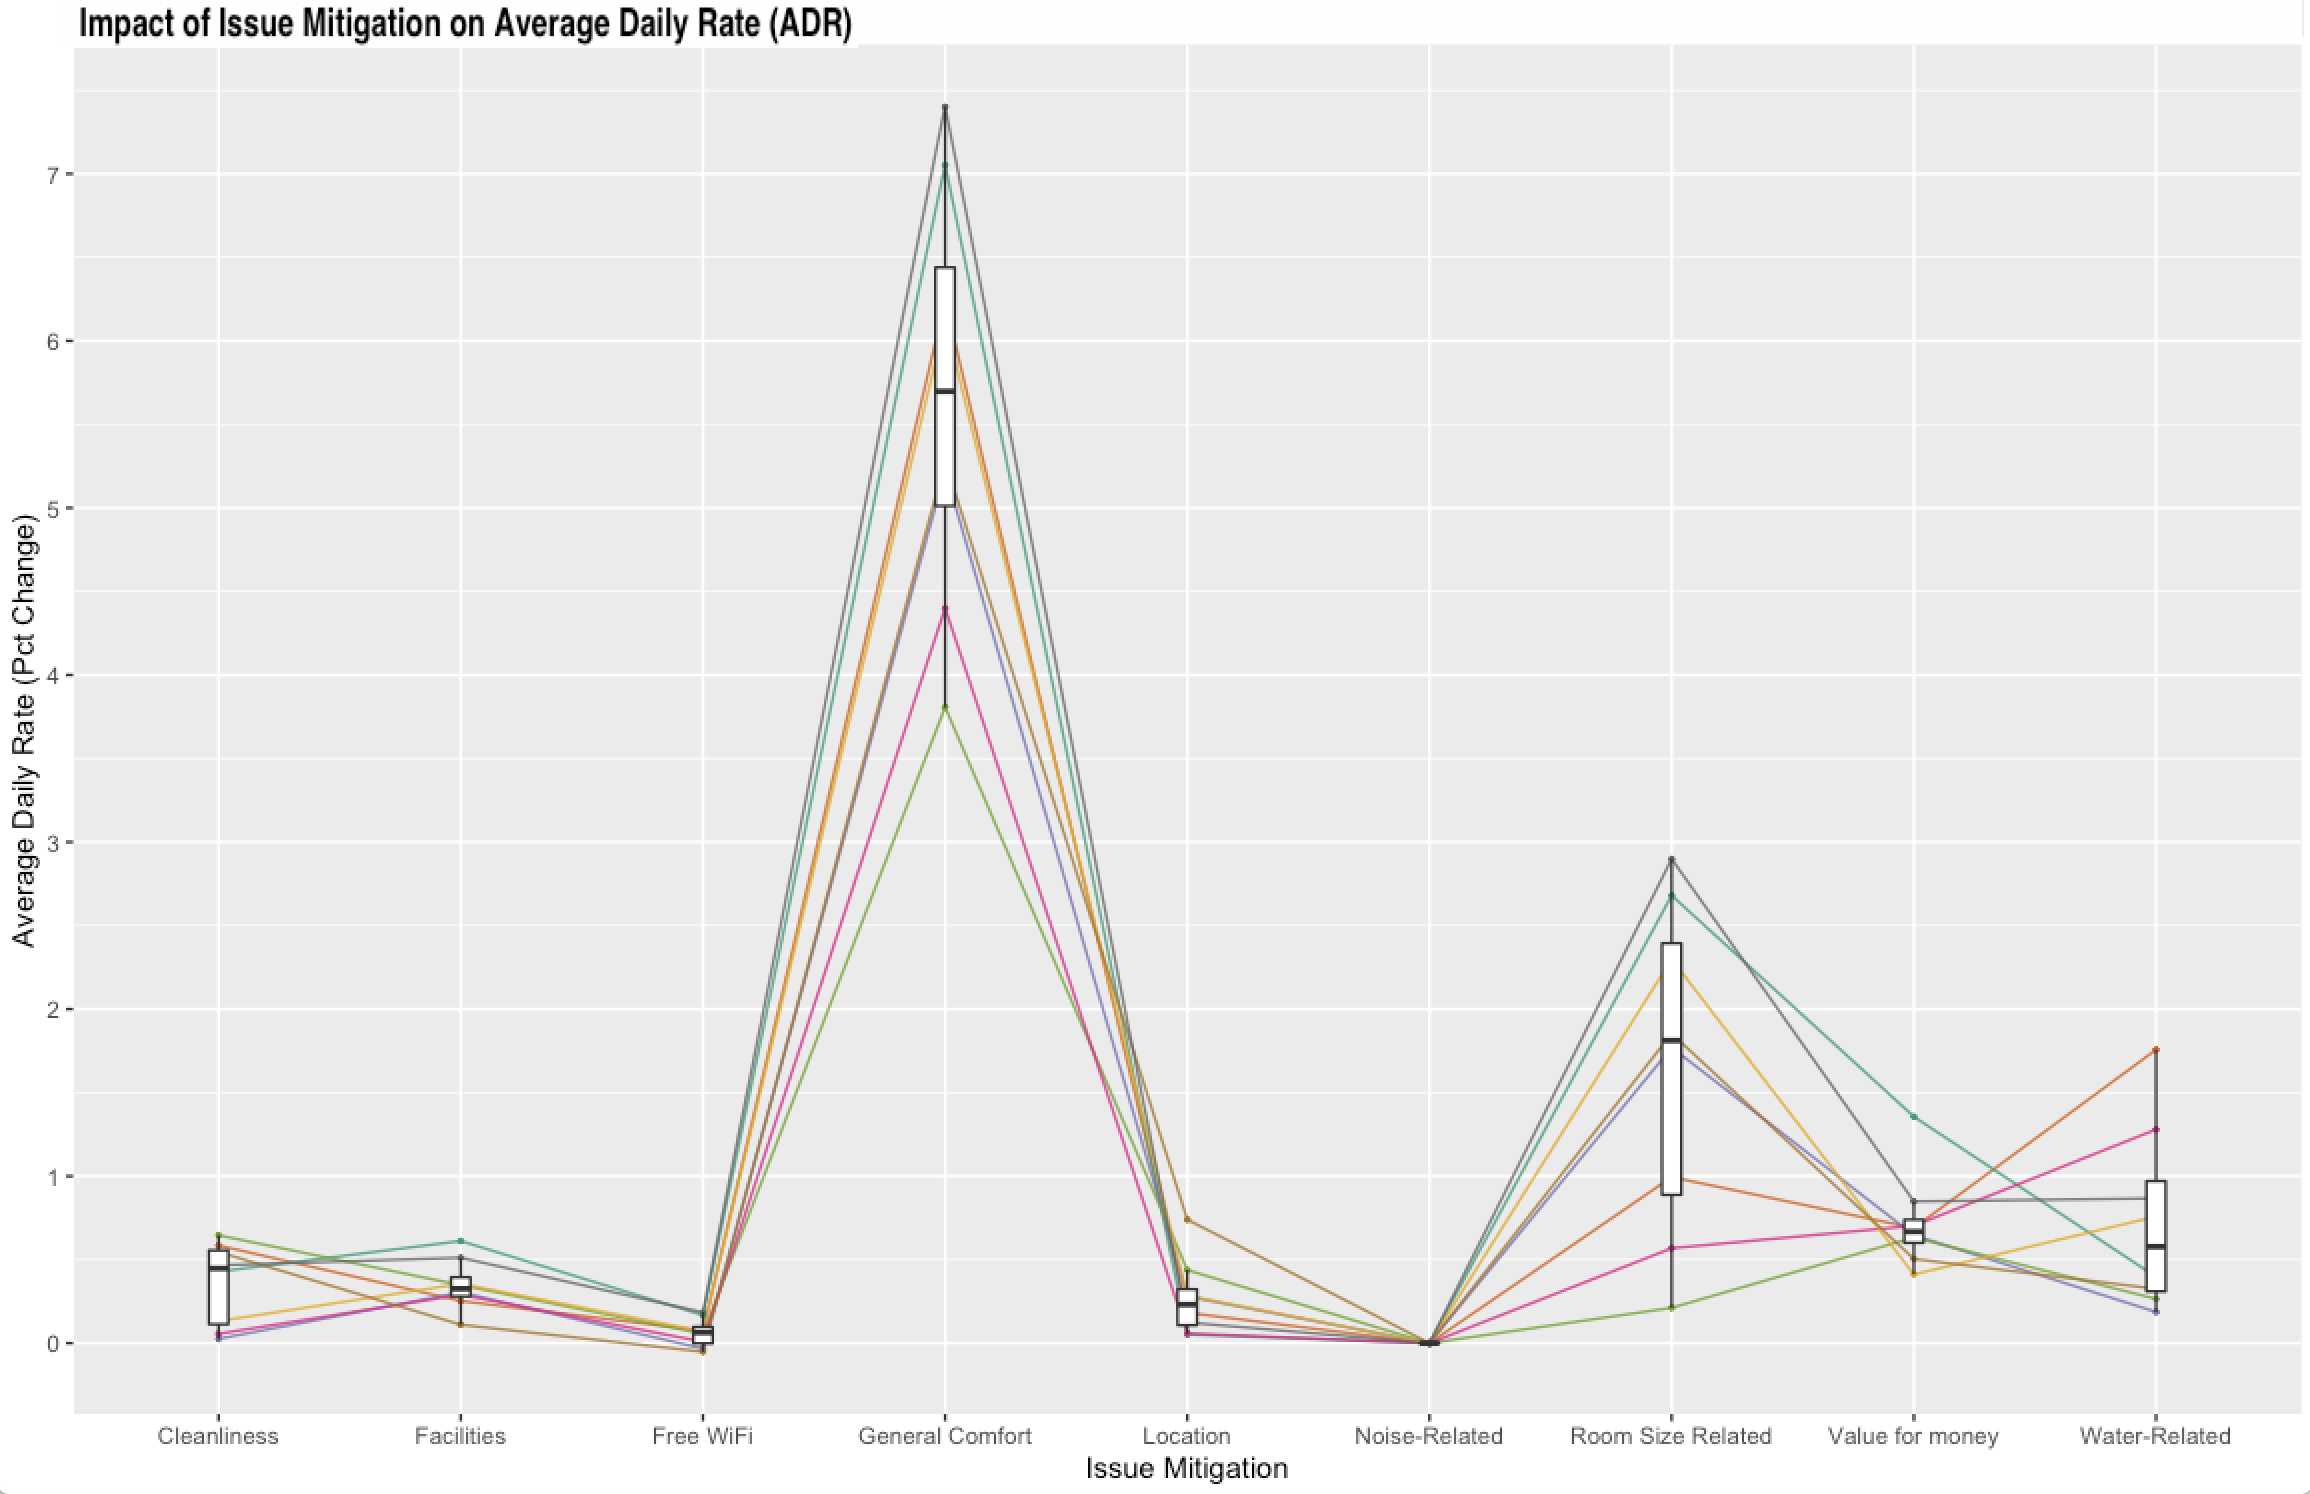
\includegraphics[width=7.2cm]{images/testimage3_2}}}%
	\caption{Floating Images}%
	\label{fig:floatimage}%
\end{figure*}


\subsection{Miscellaneous}

\subsubsection{Hyperlinks}
% HYPERLINK
\href{https://www.cnn.com}{A hyperlink to CNN.com}

% TO ADD A REFERENCE TO A SECTION
This is a section labelled as "sec1"
\label{sec:sec1}

This is a reference to the section sec1: \ref{sec:sec1}

\fbox{\begin{minipage}{43em}
		\textbf{Using fbox and minipage}\\
Text enclosed in a box
\end{minipage}}

% CODE
\subsubsection{Python Code Formatting}
\lstinputlisting[language=Python]{code/test.py}

\subsubsection{R Code Formatting}
\lstinputlisting[language=R]{code/test.R}

\subsubsection{Tables and Equations}

Examples with tables, caption centering, equations and aligned equations.

\begin{table}[!ht]
	\centering
	\captionsetup{justification=centering}
	\begin{tabular}{l|llrr}
		%		\hline
		\textbf{Model}            & \textbf{Parameter} & \textbf{Best Fit}              & \textbf{Train RMSE}             & \textbf{Test RMSE}               \\ \hline
		Linear Regression         & -                  & -                              & \rupee16,758,137 & \rupee57,778,006  \\ \hline
		Random GLM                & maxOrder           & maxInt.Order = 2        & \rupee15,551,472 & \rupee100,219,602 \\ \hline
		SVM RBF Kernel            & C, Sigma           & sigma = 26.76, C = 4     & \rupee17,075,271 & \rupee34,932,347  \\ \hline
		KNN                       & k                  & k = 5                          & \rupee12,255,888 & \rupee54,935,698  \\ \hline
		RandomForest              & mtry               & mtry = 2                       & \rupee8,724,815  & \rupee53,453,612  \\ \hline
		\rowcolor[HTML]{EFEFEF} 
		XGBoost & misc*              & max\_depth = 3, $\eta$ = 0.3, $\gamma$ = 0      & \rupee4,924,454  & \rupee65,211,901  \\ \hline
	\end{tabular}
	\caption{This is a table}
	\label{tab:state_pred}
\end{table}

Split Line in Equations
\begin{equation}
\begin{split}
\label{eqn:natsec}
ln(GVA_{Sector}) = \beta_1ln(SumOfLights)_{t}+\beta_2ln(SumElectricity)_t +\\ \beta_3ln(SumOfLightsSq)_{t} + \beta_4ln(Population)_{t} +
\alpha_i + u_{it}
\end{split}
\end{equation}

Aligned Equations
$$
\begin{aligned}
y_t &= 10.3009 -0.0042x_L - 0.0045x_B - 0.0032x_c -0.0046x_{d1} + \ldots + 0.0176x_{d6} + \eta_t \\
\eta_t &= 0.9146\eta_{t-1} + \epsilon_t -0.5015\epsilon_{t-1}\\
\epsilon_t &= \sim \text{NID}(0,0.003443)
\end{aligned}
$$

\subsubsection{Citations}
This template uses Bath BibTeX: \hyperlink{https://ctan.org/pkg/bath-bst?lang=en}{https://ctan.org/pkg/bath-bst?lang=en}

See: \hyperlink{https://github.com/alex-ball/bathbib/tree/master/bst}{https://github.com/alex-ball/bathbib/tree/master/bst}

This is a citation \citep{Elvidge_Baugh_Zhizhin_Hsu_Ghosh_2017} using \texttt{citep}.

This is a citation \cite{Tibshirani_1996} using \texttt{cite}

%TC:endignore
\pagebreak
\end{verbatim}
{\color{red} \rule{\linewidth}{0.5mm}}

\textcolor{red}{\textbf{FONT USAGE}}

The Arial font is recommended for the Individual Research Report. However, this needs to be installed manually as discussed in this document. For Overleaf, Helvetica has been used. If you are able to install Arial, comment the line \texttt{usepackage[scaled]\{helvet\}} and uncomment \texttt{usepackage\{uarial\}}.

{\color{red} \rule{\linewidth}{0.5mm}}

\textbf{FORMATTING AND PAGE NUMBERING CONVENTIONS USED}

\begin{itemize}
	\item Geometry
	\begin{itemize}
		\item left-hand margin of 4 cm;
		\item right-hand margin of 2.5cm (1 inch);
		\item top margin 2.5cm (1 inch);
		\item bottom margin 2.5cm (1 inch).
	\end{itemize}
	\begin{itemize}
		\item The Synopsis, Acknowledgements, List of Contents and Notation should be numbered with upper case Roman Numerals.
		\item The main text, starting with the first page of the first chapter (or Introduction) should be numbered, starting with page 1, using Arabic Numerals, through to the end of the references.
		\item \textbf{Appendices should be numbered using lower case Roman Numerals. -- Check to make sure this is what is needed. If not comment \texttt{\\pagenumbering\{roman\}} in template before Appendix}
	\end{itemize}
	\item Pages must be numbered at the bottom centre of the page.
	\item The title page should be blank.
\end{itemize}

\subsection{Prerequisites}

There are 2 primary pre-requisites: First, to install the Bath BibTeX style and second to install the Arial font. Note that if Arial cannot be installed, it may be possible to use Helvetica if the department agrees 

\textbf{1. Install the Bath BibTeX style (See Included Folder)}

\textbf{2. Install Font Arial}: See \hyperlink{https://www.tug.org/fonts/getnonfreefonts/}{https://www.tug.org/fonts/getnonfreefonts/} and 

\textbf{Notes from \hyperlink{https://tex.stackexchange.com/questions/37120/how-can-i-install-uarial-sty-on-a-mac}{Install uarial on a Mac} question on Stackexchange: }

The font can be easily installed via the script getnonfreefonts. It is available at tug.org: \hyperlink{http://www.tug.org/fonts/getnonfreefonts/}{getnonfreefonts}. I tried the installation of \hyperlink{http://www.tug.org/fonts/getnonfreefonts/install-getnonfreefonts}{getnonfreefonts} on my Mac.

\begin{itemize}
	\item Install MacTeX 
	\item Download the installation script. Open the terminal and go to the folder Download
	
	\texttt{cd Download}
	\item Run the installation: \texttt{sudo texlua install-getnonfreefonts}
	
	The installation finished and the scipts with their execute files getnonefreefonts and getnonfreefonts-sys are now located at \texttt{/usr/local/texlive/2011/bin/x86\_64-darwin/}
	
	\item Now you can run the script \texttt{sudo getnonfreefonts-sys -a}
\end{itemize}

\subsection{Images}
\begin{figure*}[!ht]
	\centering
	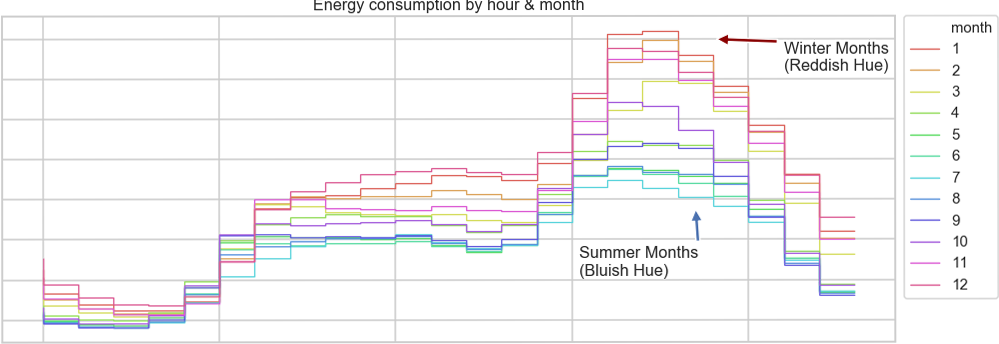
\includegraphics[width=16cm]{images/testimage1}
	\caption{This is an image}
	\label{fig:testimage1}
\end{figure*}

\begin{figure*}[!ht]
	\centering
	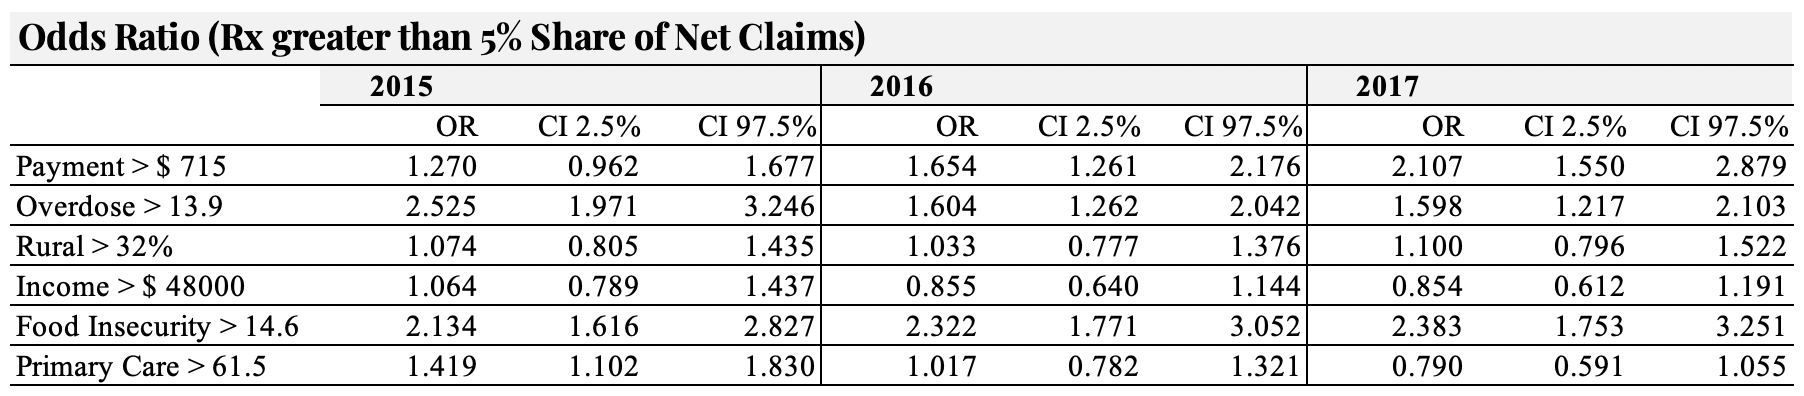
\includegraphics[width=16cm]{images/testimage2}
	%	\caption{Round 1 Blue Strategy to increase Market Share}
	\captionof{table}[This is a table shown as an image]{This is a table shown as an image}
	\label{fig:testimage2}
\end{figure*}

\begin{figure*}[!ht]
	\centering
	\subfloat[A floating image]{{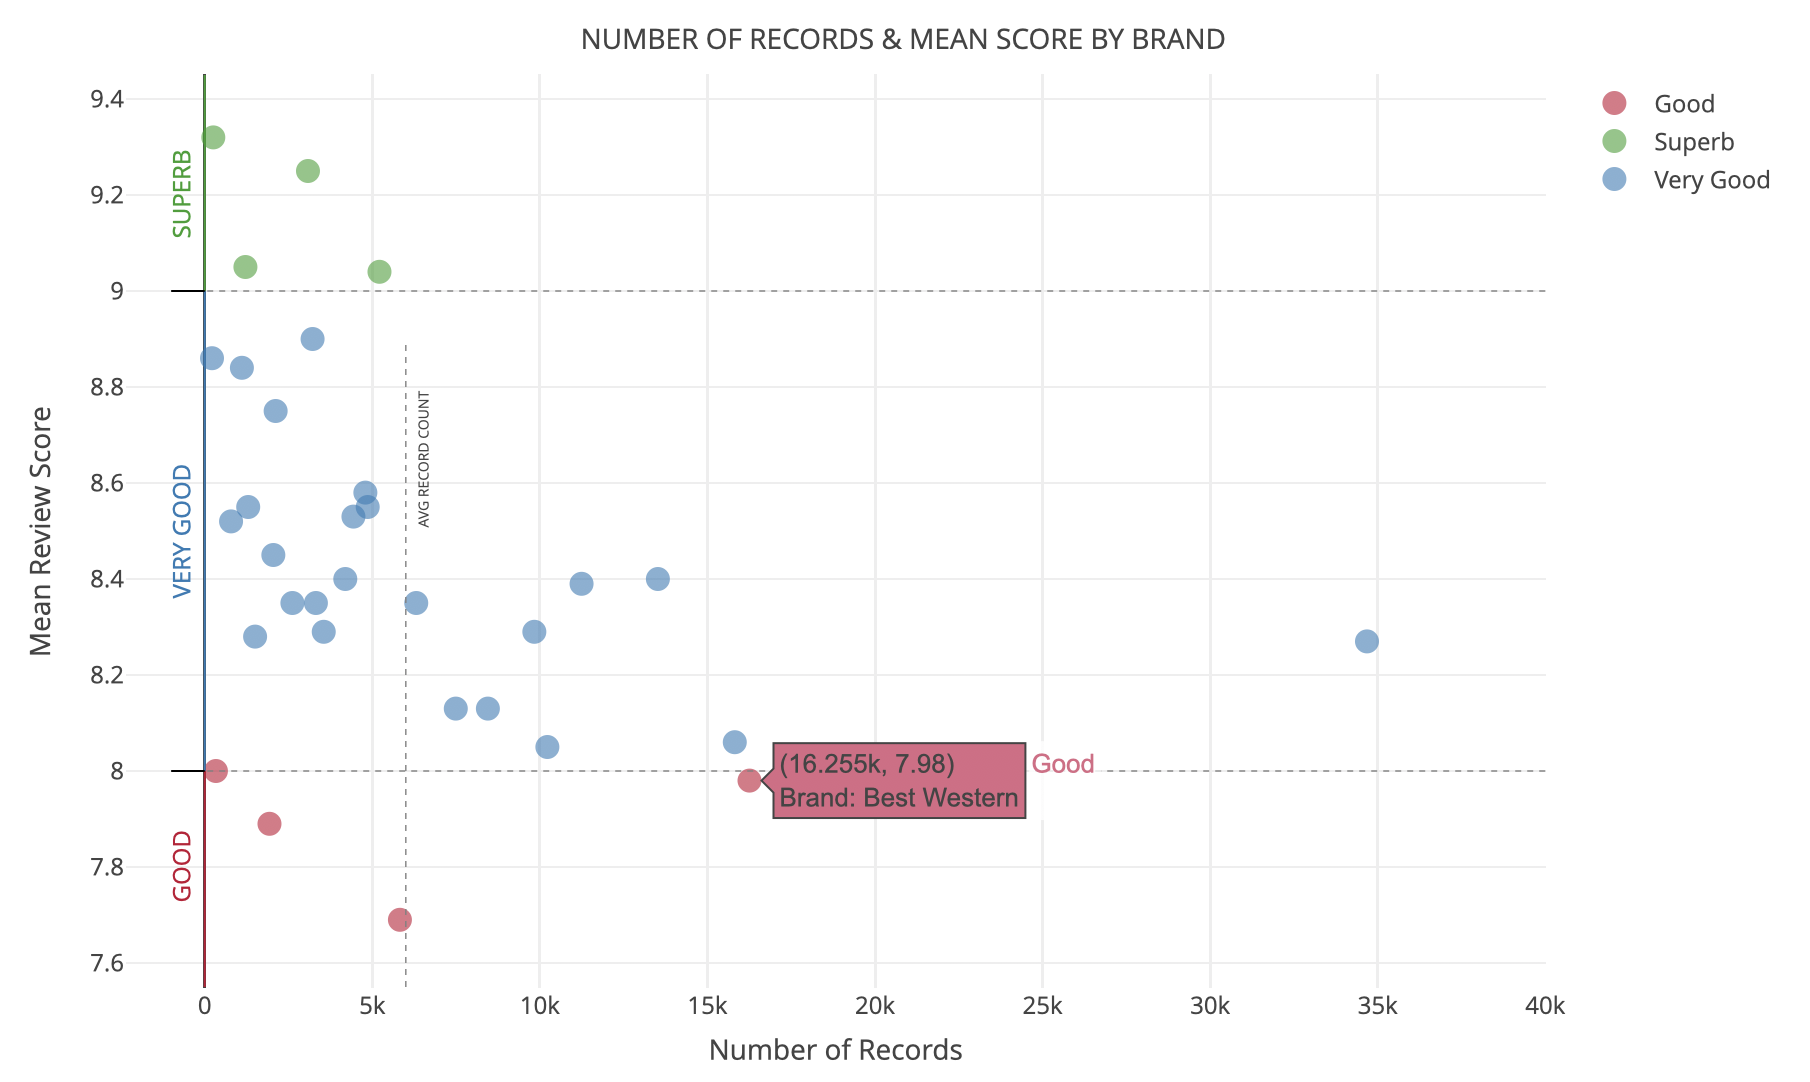
\includegraphics[width=7.2cm]{images/testimage3_1} }}%
	%	\qquad
	\subfloat[Another image ]{{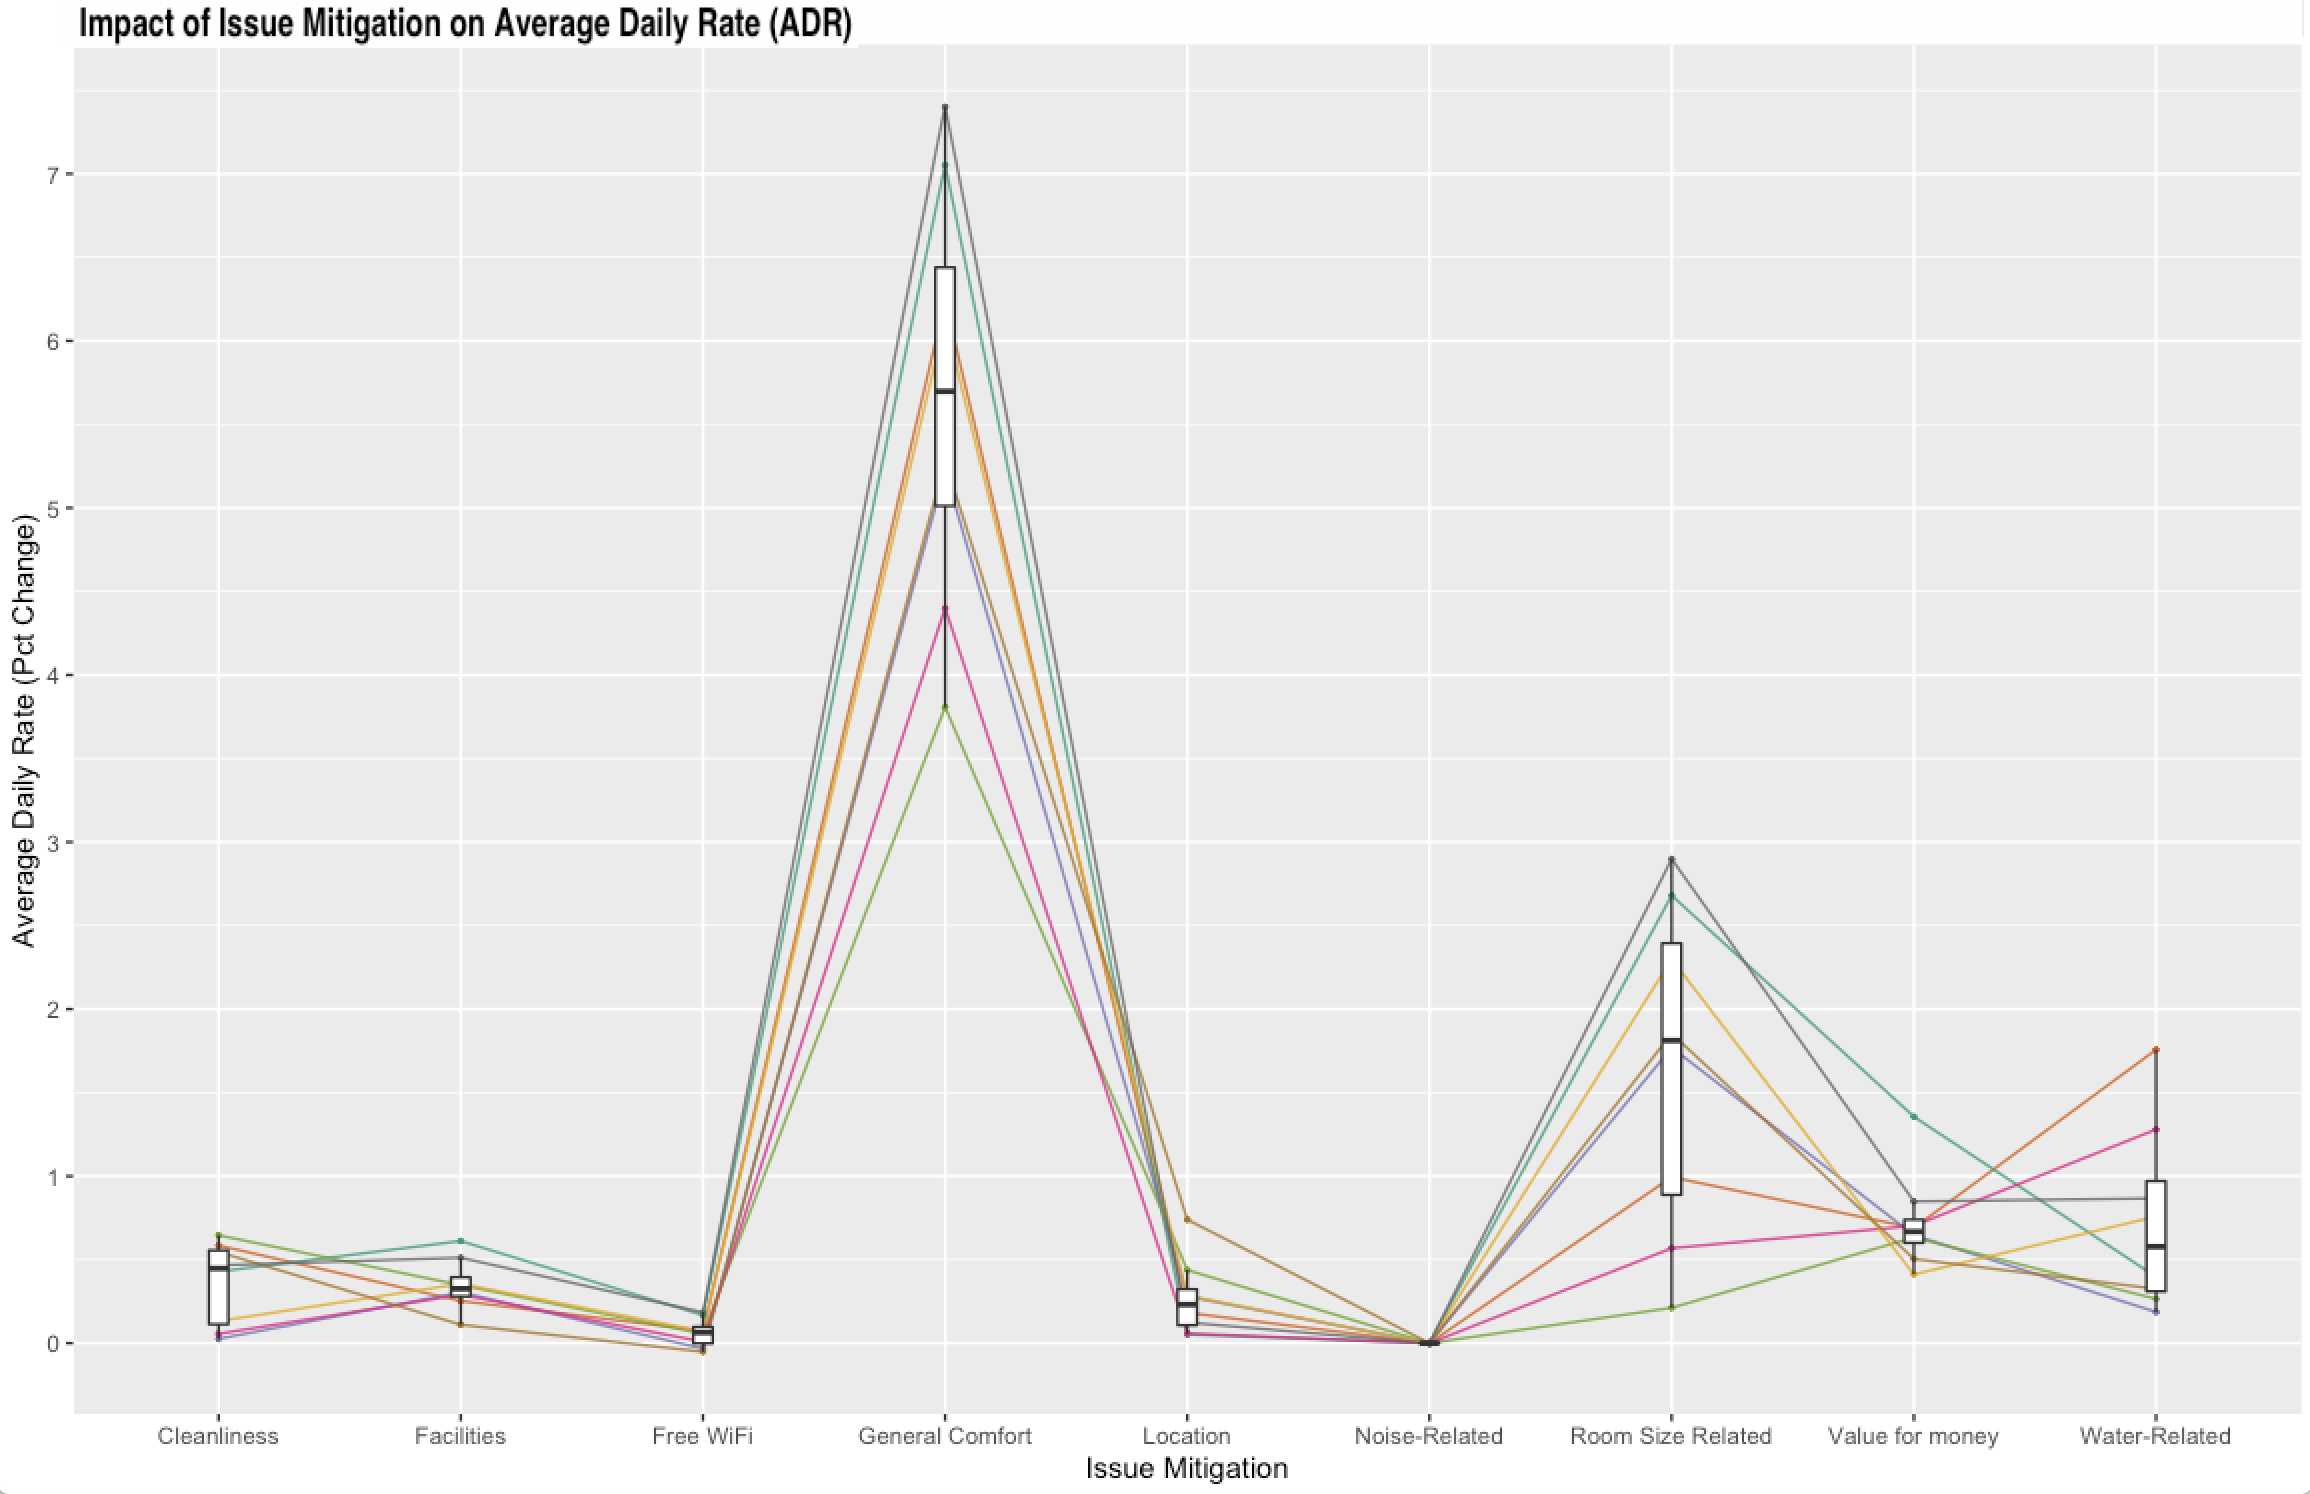
\includegraphics[width=7.2cm]{images/testimage3_2}}}%
	\caption{Floating Images}%
	\label{fig:floatimage}%
\end{figure*}


\subsection{Miscellaneous}

\subsubsection{Hyperlinks}
% HYPERLINK
\href{https://www.cnn.com}{A hyperlink to CNN.com}

% TO ADD A REFERENCE TO A SECTION
This is a section labelled as "sec1"
\label{sec:sec1}

This is a reference to the section sec1: \ref{sec:sec1}

\fbox{\begin{minipage}{43em}
		\textbf{Using fbox and minipage}\\
Text enclosed in a box
\end{minipage}}

% CODE
\subsubsection{Python Code Formatting}
\lstinputlisting[language=Python]{code/test.py}

\subsubsection{R Code Formatting}
\lstinputlisting[language=R]{code/test.R}

\subsubsection{Tables and Equations}

Examples with tables, caption centering, equations and aligned equations.

\begin{table}[!ht]
	\centering
	\captionsetup{justification=centering}
	\begin{tabular}{l|llrr}
		%		\hline
		\textbf{Model}            & \textbf{Parameter} & \textbf{Best Fit}              & \textbf{Train RMSE}             & \textbf{Test RMSE}               \\ \hline
		Linear Regression         & -                  & -                              & \rupee16,758,137 & \rupee57,778,006  \\ \hline
		Random GLM                & maxOrder           & maxInt.Order = 2        & \rupee15,551,472 & \rupee100,219,602 \\ \hline
		SVM RBF Kernel            & C, Sigma           & sigma = 26.76, C = 4     & \rupee17,075,271 & \rupee34,932,347  \\ \hline
		KNN                       & k                  & k = 5                          & \rupee12,255,888 & \rupee54,935,698  \\ \hline
		RandomForest              & mtry               & mtry = 2                       & \rupee8,724,815  & \rupee53,453,612  \\ \hline
		\rowcolor[HTML]{EFEFEF} 
		XGBoost & misc*              & max\_depth = 3, $\eta$ = 0.3, $\gamma$ = 0      & \rupee4,924,454  & \rupee65,211,901  \\ \hline
	\end{tabular}
	\caption{This is a table}
	\label{tab:state_pred}
\end{table}

Split Line in Equations
\begin{equation}
\begin{split}
\label{eqn:natsec}
ln(GVA_{Sector}) = \beta_1ln(SumOfLights)_{t}+\beta_2ln(SumElectricity)_t +\\ \beta_3ln(SumOfLightsSq)_{t} + \beta_4ln(Population)_{t} +
\alpha_i + u_{it}
\end{split}
\end{equation}

Aligned Equations
$$
\begin{aligned}
y_t &= 10.3009 -0.0042x_L - 0.0045x_B - 0.0032x_c -0.0046x_{d1} + \ldots + 0.0176x_{d6} + \eta_t \\
\eta_t &= 0.9146\eta_{t-1} + \epsilon_t -0.5015\epsilon_{t-1}\\
\epsilon_t &= \sim \text{NID}(0,0.003443)
\end{aligned}
$$

\subsubsection{Citations}
This template uses Bath BibTeX: \hyperlink{https://ctan.org/pkg/bath-bst?lang=en}{https://ctan.org/pkg/bath-bst?lang=en}

See: \hyperlink{https://github.com/alex-ball/bathbib/tree/master/bst}{https://github.com/alex-ball/bathbib/tree/master/bst}

This is a citation \citep{Elvidge_Baugh_Zhizhin_Hsu_Ghosh_2017} using \texttt{citep}.

This is a citation \cite{Tibshirani_1996} using \texttt{cite}

%TC:endignore
\pagebreak
\end{verbatim}
{\color{red} \rule{\linewidth}{0.5mm}}

\textcolor{red}{\textbf{FONT USAGE}}

The Arial font is recommended for the Individual Research Report. However, this needs to be installed manually as discussed in this document. For Overleaf, Helvetica has been used. If you are able to install Arial, comment the line \texttt{usepackage[scaled]\{helvet\}} and uncomment \texttt{usepackage\{uarial\}}.

{\color{red} \rule{\linewidth}{0.5mm}}

\textbf{FORMATTING AND PAGE NUMBERING CONVENTIONS USED}

\begin{itemize}
	\item Geometry
	\begin{itemize}
		\item left-hand margin of 4 cm;
		\item right-hand margin of 2.5cm (1 inch);
		\item top margin 2.5cm (1 inch);
		\item bottom margin 2.5cm (1 inch).
	\end{itemize}
	\begin{itemize}
		\item The Synopsis, Acknowledgements, List of Contents and Notation should be numbered with upper case Roman Numerals.
		\item The main text, starting with the first page of the first chapter (or Introduction) should be numbered, starting with page 1, using Arabic Numerals, through to the end of the references.
		\item \textbf{Appendices should be numbered using lower case Roman Numerals. -- Check to make sure this is what is needed. If not comment \texttt{\\pagenumbering\{roman\}} in template before Appendix}
	\end{itemize}
	\item Pages must be numbered at the bottom centre of the page.
	\item The title page should be blank.
\end{itemize}

\subsection{Prerequisites}

There are 2 primary pre-requisites: First, to install the Bath BibTeX style and second to install the Arial font. Note that if Arial cannot be installed, it may be possible to use Helvetica if the department agrees 

\textbf{1. Install the Bath BibTeX style (See Included Folder)}

\textbf{2. Install Font Arial}: See \hyperlink{https://www.tug.org/fonts/getnonfreefonts/}{https://www.tug.org/fonts/getnonfreefonts/} and 

\textbf{Notes from \hyperlink{https://tex.stackexchange.com/questions/37120/how-can-i-install-uarial-sty-on-a-mac}{Install uarial on a Mac} question on Stackexchange: }

The font can be easily installed via the script getnonfreefonts. It is available at tug.org: \hyperlink{http://www.tug.org/fonts/getnonfreefonts/}{getnonfreefonts}. I tried the installation of \hyperlink{http://www.tug.org/fonts/getnonfreefonts/install-getnonfreefonts}{getnonfreefonts} on my Mac.

\begin{itemize}
	\item Install MacTeX 
	\item Download the installation script. Open the terminal and go to the folder Download
	
	\texttt{cd Download}
	\item Run the installation: \texttt{sudo texlua install-getnonfreefonts}
	
	The installation finished and the scipts with their execute files getnonefreefonts and getnonfreefonts-sys are now located at \texttt{/usr/local/texlive/2011/bin/x86\_64-darwin/}
	
	\item Now you can run the script \texttt{sudo getnonfreefonts-sys -a}
\end{itemize}

\subsection{Images}
\begin{figure*}[!ht]
	\centering
	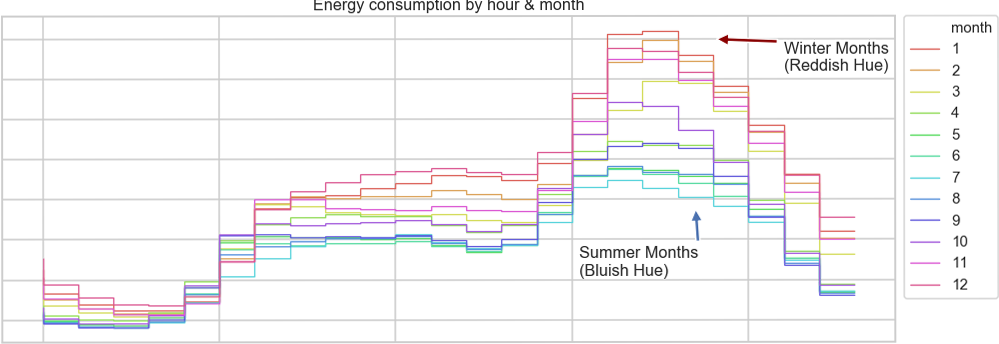
\includegraphics[width=16cm]{images/testimage1}
	\caption{This is an image}
	\label{fig:testimage1}
\end{figure*}

\begin{figure*}[!ht]
	\centering
	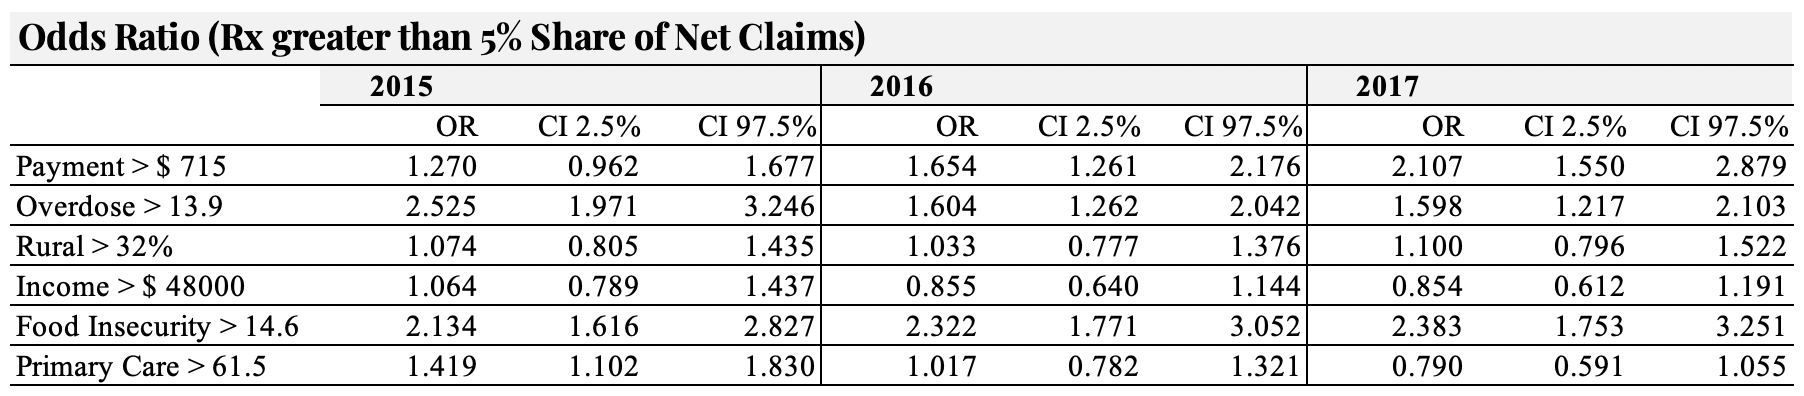
\includegraphics[width=16cm]{images/testimage2}
	%	\caption{Round 1 Blue Strategy to increase Market Share}
	\captionof{table}[This is a table shown as an image]{This is a table shown as an image}
	\label{fig:testimage2}
\end{figure*}

\begin{figure*}[!ht]
	\centering
	\subfloat[A floating image]{{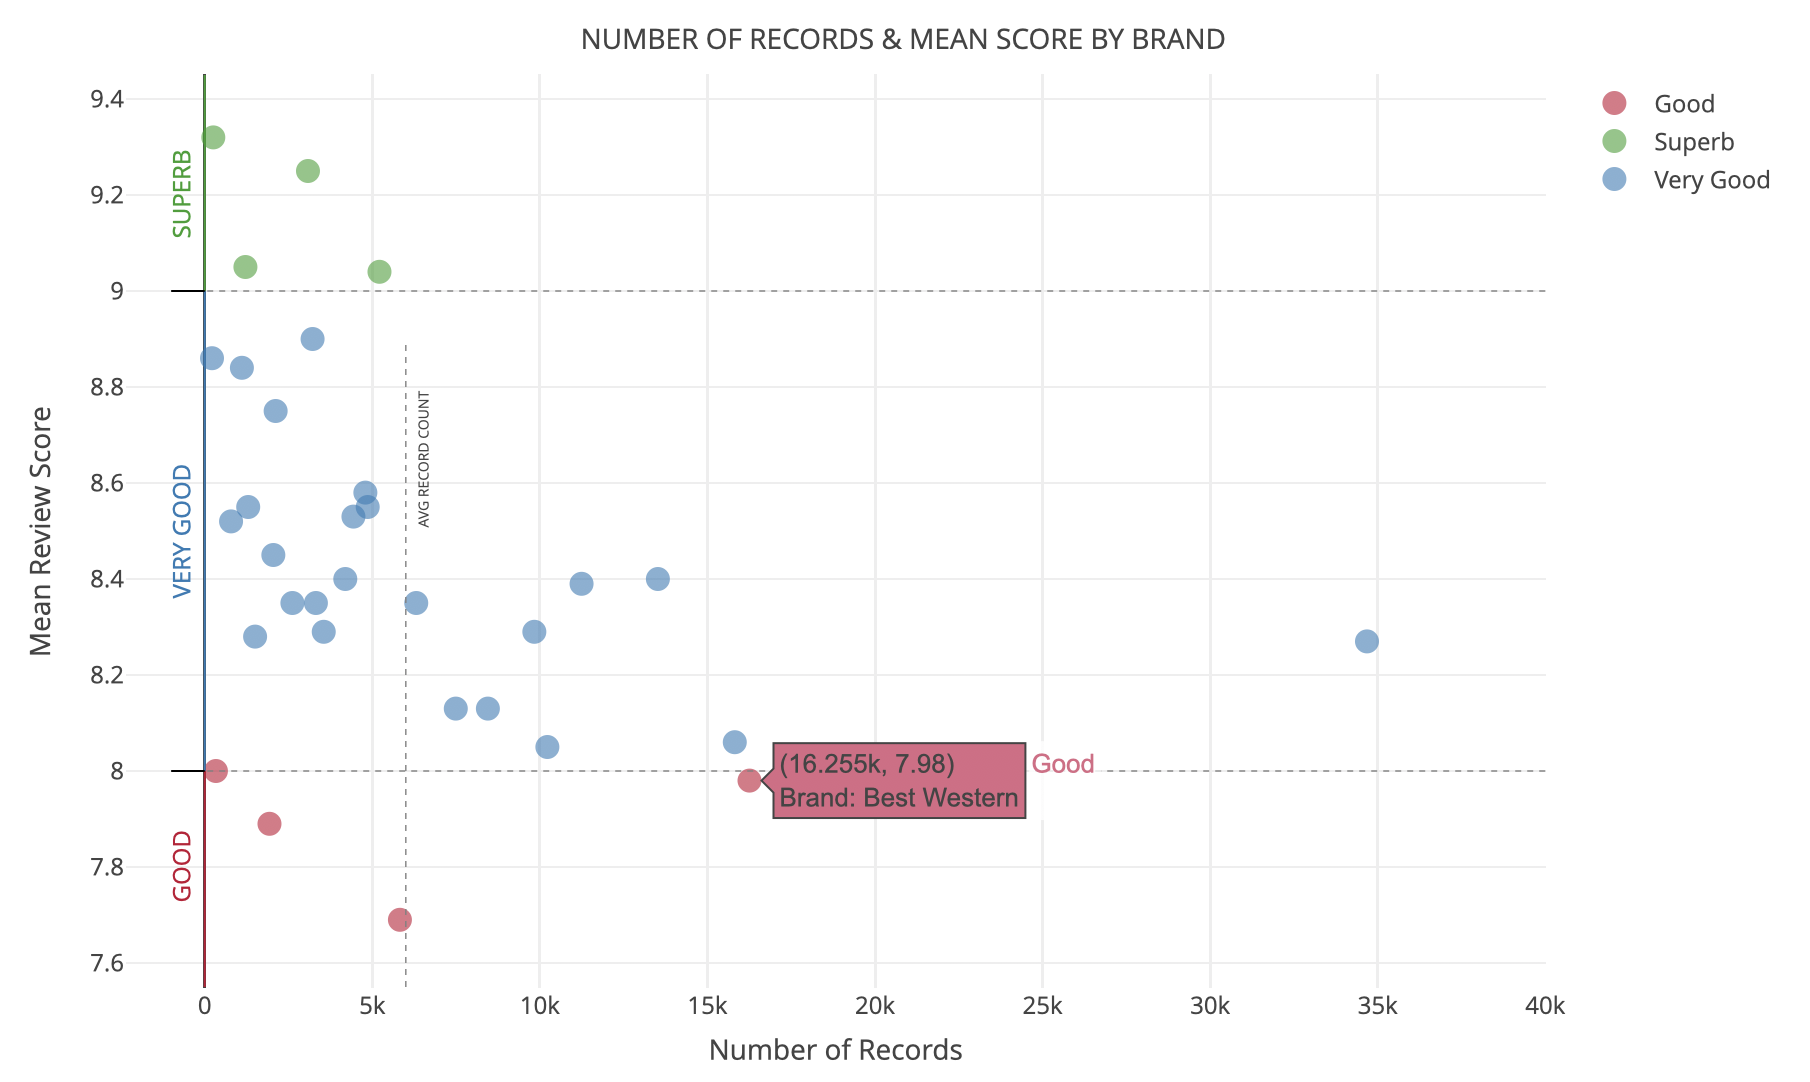
\includegraphics[width=7.2cm]{images/testimage3_1} }}%
	%	\qquad
	\subfloat[Another image ]{{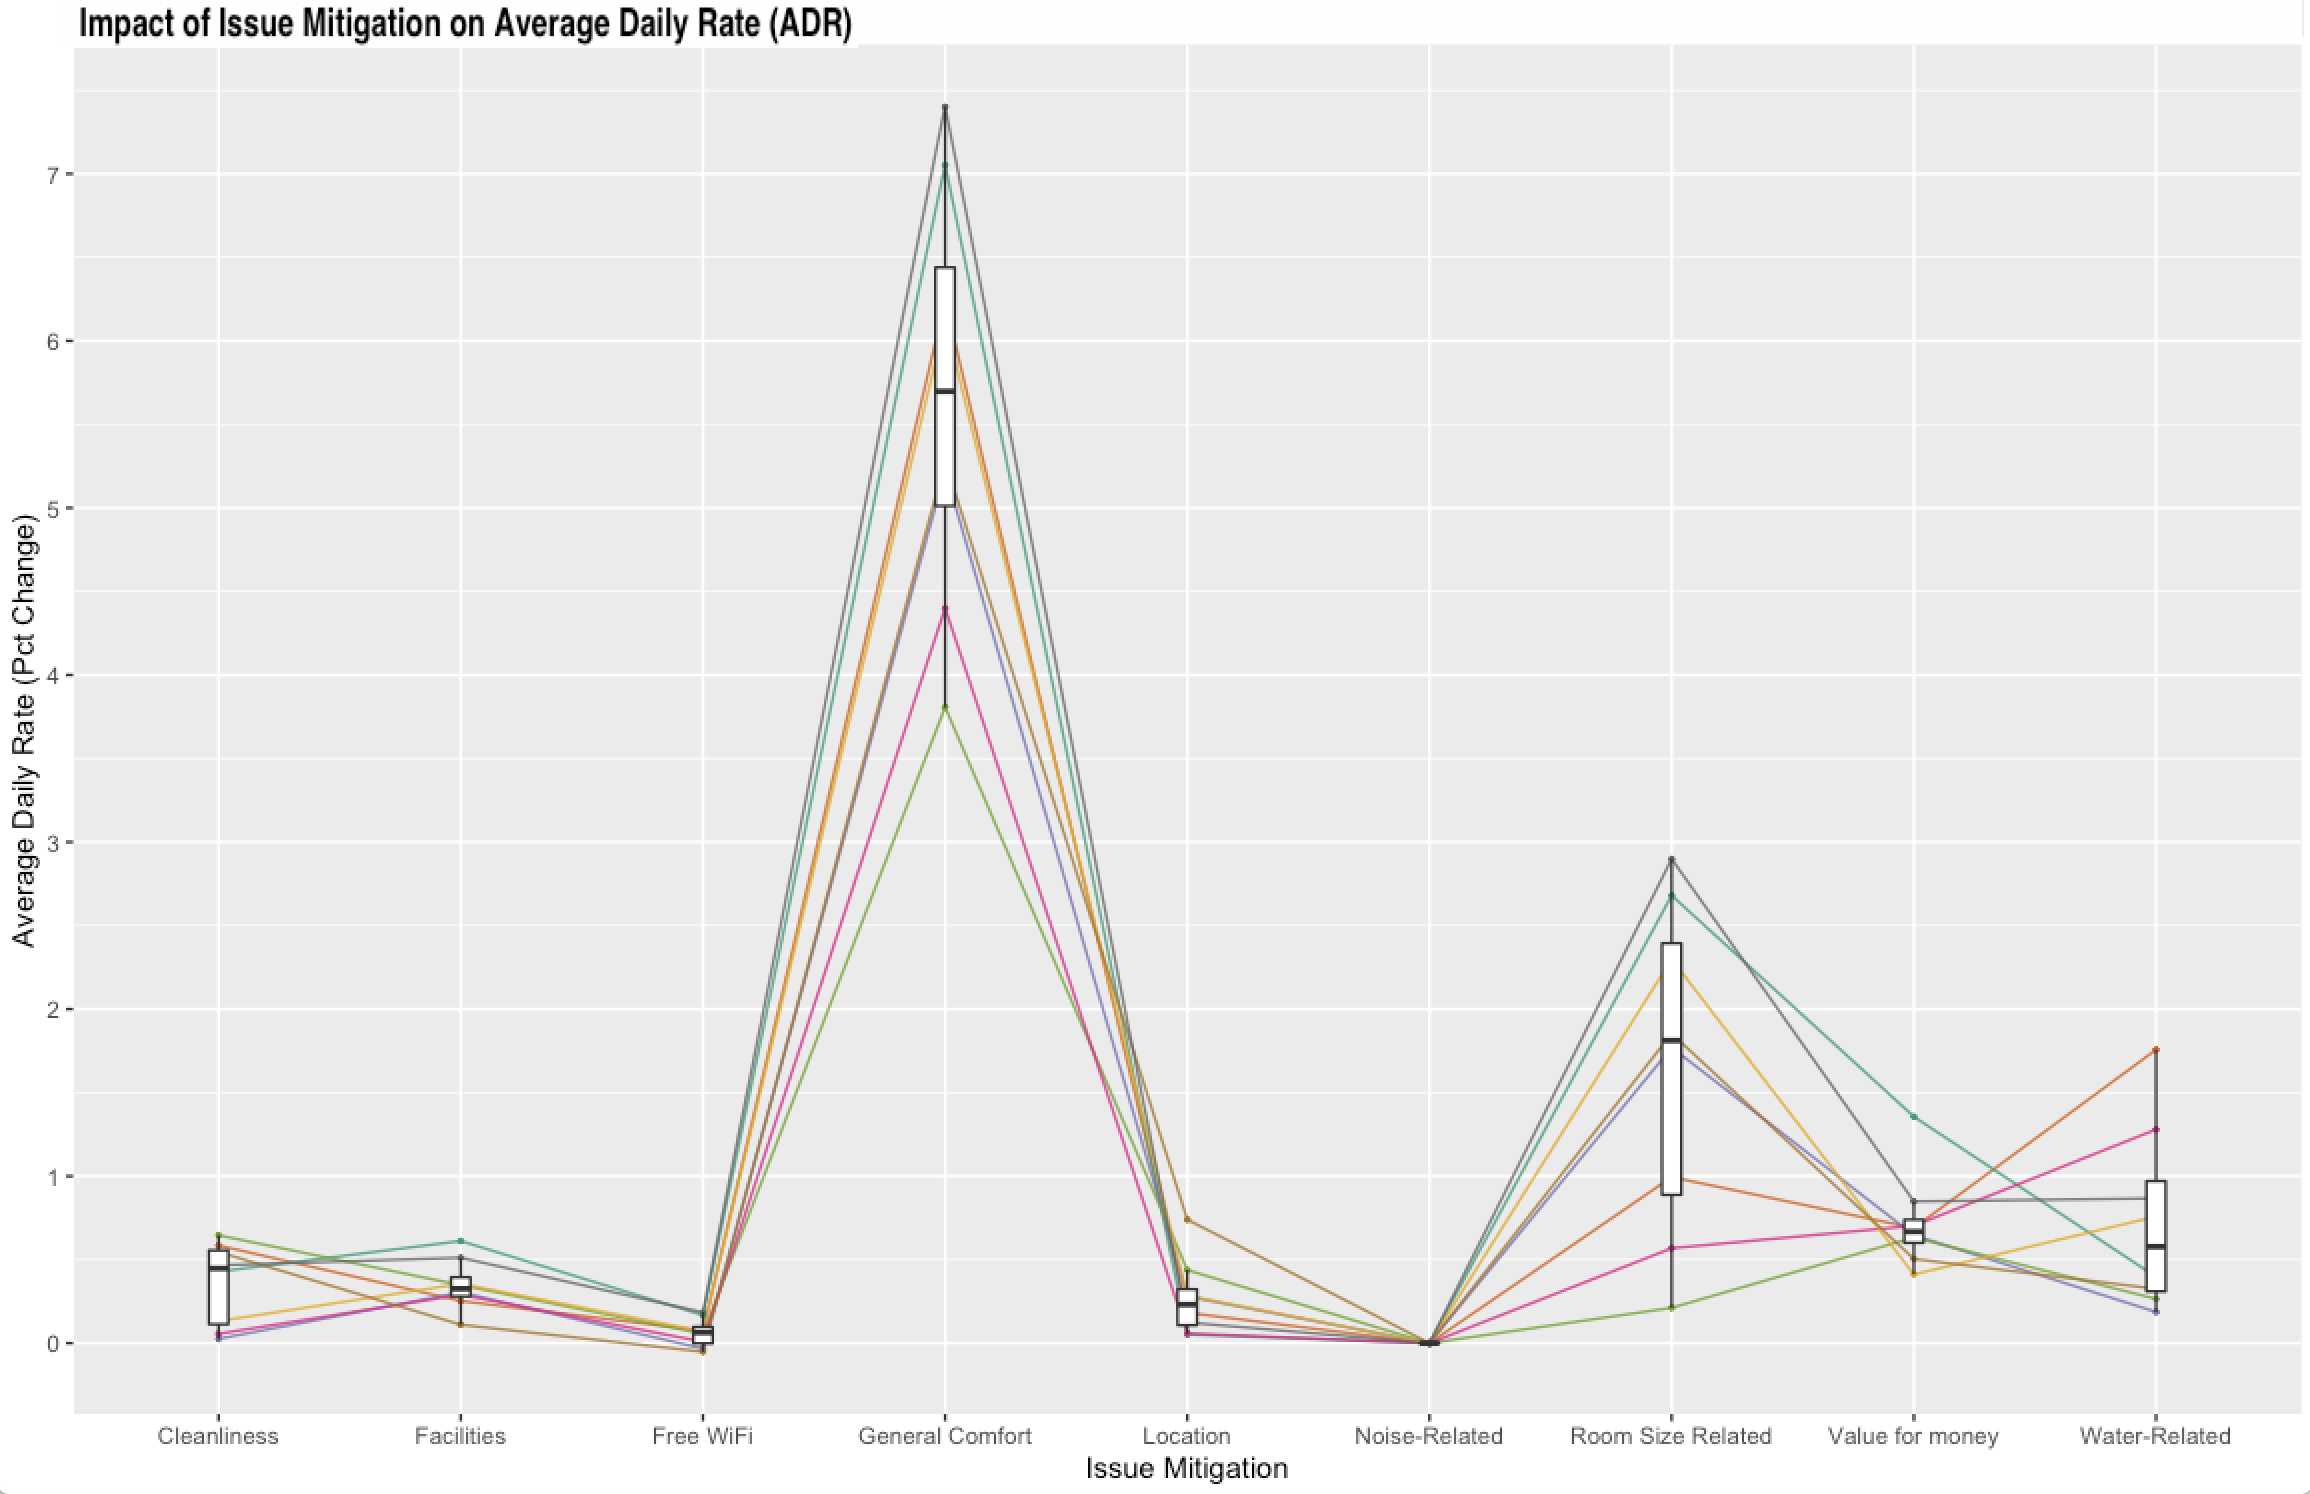
\includegraphics[width=7.2cm]{images/testimage3_2}}}%
	\caption{Floating Images}%
	\label{fig:floatimage}%
\end{figure*}


\subsection{Miscellaneous}

\subsubsection{Hyperlinks}
% HYPERLINK
\href{https://www.cnn.com}{A hyperlink to CNN.com}

% TO ADD A REFERENCE TO A SECTION
This is a section labelled as "sec1"
\label{sec:sec1}

This is a reference to the section sec1: \ref{sec:sec1}

\fbox{\begin{minipage}{43em}
		\textbf{Using fbox and minipage}\\
Text enclosed in a box
\end{minipage}}

% CODE
\subsubsection{Python Code Formatting}
\lstinputlisting[language=Python]{code/test.py}

\subsubsection{R Code Formatting}
\lstinputlisting[language=R]{code/test.R}

\subsubsection{Tables and Equations}

Examples with tables, caption centering, equations and aligned equations.

\begin{table}[!ht]
	\centering
	\captionsetup{justification=centering}
	\begin{tabular}{l|llrr}
		%		\hline
		\textbf{Model}            & \textbf{Parameter} & \textbf{Best Fit}              & \textbf{Train RMSE}             & \textbf{Test RMSE}               \\ \hline
		Linear Regression         & -                  & -                              & \rupee16,758,137 & \rupee57,778,006  \\ \hline
		Random GLM                & maxOrder           & maxInt.Order = 2        & \rupee15,551,472 & \rupee100,219,602 \\ \hline
		SVM RBF Kernel            & C, Sigma           & sigma = 26.76, C = 4     & \rupee17,075,271 & \rupee34,932,347  \\ \hline
		KNN                       & k                  & k = 5                          & \rupee12,255,888 & \rupee54,935,698  \\ \hline
		RandomForest              & mtry               & mtry = 2                       & \rupee8,724,815  & \rupee53,453,612  \\ \hline
		\rowcolor[HTML]{EFEFEF} 
		XGBoost & misc*              & max\_depth = 3, $\eta$ = 0.3, $\gamma$ = 0      & \rupee4,924,454  & \rupee65,211,901  \\ \hline
	\end{tabular}
	\caption{This is a table}
	\label{tab:state_pred}
\end{table}

Split Line in Equations
\begin{equation}
\begin{split}
\label{eqn:natsec}
ln(GVA_{Sector}) = \beta_1ln(SumOfLights)_{t}+\beta_2ln(SumElectricity)_t +\\ \beta_3ln(SumOfLightsSq)_{t} + \beta_4ln(Population)_{t} +
\alpha_i + u_{it}
\end{split}
\end{equation}

Aligned Equations
$$
\begin{aligned}
y_t &= 10.3009 -0.0042x_L - 0.0045x_B - 0.0032x_c -0.0046x_{d1} + \ldots + 0.0176x_{d6} + \eta_t \\
\eta_t &= 0.9146\eta_{t-1} + \epsilon_t -0.5015\epsilon_{t-1}\\
\epsilon_t &= \sim \text{NID}(0,0.003443)
\end{aligned}
$$

\subsubsection{Citations}
This template uses Bath BibTeX: \hyperlink{https://ctan.org/pkg/bath-bst?lang=en}{https://ctan.org/pkg/bath-bst?lang=en}

See: \hyperlink{https://github.com/alex-ball/bathbib/tree/master/bst}{https://github.com/alex-ball/bathbib/tree/master/bst}

This is a citation \citep{Elvidge_Baugh_Zhizhin_Hsu_Ghosh_2017} using \texttt{citep}.

This is a citation \cite{Tibshirani_1996} using \texttt{cite}

%TC:endignore